% !TEX program = xelatex
\documentclass[oneside]{ctexbook}
\usepackage{hyperref}
\hypersetup{
    colorlinks=true,
    linkcolor=blue,
    filecolor=magenta,      
    urlcolor=cyan,
    pdftitle={数据结构与算法分析},
    pdfpagemode=FullScreen,
}
\setcounter{tocdepth}{4}
\setcounter{secnumdepth}{4}
\usepackage{multirow}
\usepackage{xcolor}
\usepackage{graphicx}
\usepackage{tikz}
\usepackage{pgfplots}
\usepackage{amsmath}
\usepackage[most]{tcolorbox}
\tcbuselibrary{minted,skins,breakable}

\tcbuselibrary{theorems}

\newtcbtheorem[number within=chapter]{mydefinition}{定义}{colback=white!5,colframe=red!35!black,fonttitle=\bfseries}{th}
\newtcbtheorem[number within=chapter]{mytheorem}{定理}{colback=white!5,colframe=blue!35!black,fonttitle=\bfseries}{th}
\newtcbtheorem[number within=chapter]{myproof}{证明}{colback=white!5,colframe=yellow!35!black,fonttitle=\bfseries}{th}

\newtcblisting[auto counter, number within=chapter]{myjava}[2]{
    listing engine=minted,
    minted style=colorful,
    minted language=java,
    minted options={
        fontsize=\small,
        breaklines,
        autogobble,
        linenos,
        numbersep=3mm,
        mathescape=true,
        texcomments
    },
    colback=blue!5!white,
    colframe=blue!75!black,
    title={程序 \thetcbcounter: #2},
    listing only,
    breakable,
    left=5mm,
    enhanced,
    overlay={
        \begin{tcbclipinterior}
            \fill[red!20!blue!20!white] (frame.south west) rectangle ([xshift=5mm]frame.north west);
        \end{tcbclipinterior}
    },
    #1
}

\newtcblisting{mytext}{
    listing engine=minted,
    minted style=colorful,
    minted language=text,
    minted options={
        fontsize=\small,
        breaklines,
        autogobble,
        numbersep=3mm,
        mathescape=true
    },
    colback=gray!5!white,
    colframe=gray!75!black,
    listing only,
    breakable,
    left=5mm,
    enhanced,
}

\newtcolorbox[blend into=tables]{mytable}[2][]{float=htb, halign=center, title={#2}, every float=\centering, #1}
\newtcolorbox[blend into=figures]{myfigure}[2][]{float=htb, halign=center, title={#2}, every float=\centering, #1}

\newtcolorbox{marker}[1][]{enhanced,
  before skip=2mm,after skip=3mm,
  boxrule=0.4pt,left=5mm,right=2mm,top=1mm,bottom=1mm,
  colback=yellow!50,
  colframe=yellow!20!black,
  sharp corners,rounded corners=southeast,arc is angular,arc=3mm,
  underlay={%
    \path[fill=tcbcolback!80!black] ([yshift=3mm]interior.south east)--++(-0.4,-0.1)--++(0.1,-0.2);
    \path[draw=tcbcolframe,shorten <=-0.05mm,shorten >=-0.05mm] ([yshift=3mm]interior.south east)--++(-0.4,-0.1)--++(0.1,-0.2);
    \path[fill=yellow!50!black,draw=none] (interior.south west) rectangle node[white]{\Huge\bfseries !} ([xshift=4mm]interior.north west);
    },
  drop fuzzy shadow,#1}

\colorlet{LightGray}{blue!5!white}

\newmintinline{java}{
    bgcolor=LightGray,
    fontsize=\small,
}

\newtcbox{\myleetcode}[1][green]{enhanced,nobeforeafter,tcbox raise base,boxrule=0.4pt,top=0mm,bottom=0mm,
  right=0mm,left=4mm,arc=1pt,boxsep=2pt,before upper={\vphantom{dlg}},
  colframe=#1!50!black,coltext=green!25!black,colback=#1!10!white,
  overlay={\begin{tcbclipinterior}\fill[green!75!blue!50!white] (frame.south west)
    rectangle node[text=white,font=\sffamily\bfseries\tiny,rotate=90] {力扣} ([xshift=4mm]frame.north west);\end{tcbclipinterior}}}

\title{数据结构与算法分析}
\author{左元}

\begin{document}

\maketitle
\tableofcontents

\chapter{引论}

在本章中, 我们将阐述本课程的目的和目标并简要复习离散数学以及程序设计的一些概念. 我们将要:

\begin{itemize}
    \item 看到程序对于\textbf{大量}输入数据的运行性能和程序对于\textbf{适量}输入数据的运行性能的同等重要性.
    \item 复习一些数学基础.
    \item 复习递归.
\end{itemize}

\section{算法的作用}

假设有一个整型数组, 数组大小是$N$, 我们想要找出数组中第$k$个最大的数.

这个问题我们称之为\textbf{选择问题}(selection problem).

只要我们学习过一点点编程知识, 就能想到一些解决这个问题的方法. 例如以下解法:

\begin{enumerate}
    \item 使用\textbf{冒泡排序}对数组进行降序排列.
    \item 取出排好序的数组的第$k$个元素.
\end{enumerate}

如果使用以上解法, 假设我们的数组大小是$1000$万, 我们要找的是第$500$万个最大的数. 那么以上解法需要花费至少\textbf{几天}的时间才能得到结果. 显然这不是一个好解法, 因为运行的太慢了.

后面我们会讲解另一种解法, 这种解法可以在$1$秒钟之内得到正确结果.

在许多问题当中, 一个重要的观念是: 写出一个工作程序并不够. 如果这个程序在巨大的数据集上运行, 那么运行时间就变成了重要的问题. 我们将在本课程中看到对于大量的输入如何估计程序的运行时间, 尤其是如何在写具体的代码之前就比较两个程序的运行时间. 我们还将看到彻底改进程序运行速度以及确定程序瓶颈的方法. 这些方法将使我们能够发现需要我们集中精力努力优化的那些代码片段.

\section{数学知识复习}

本节列出一些需要记忆或是能够推导出的基本公式, 并从推导过程复习基本的证明方法.

\subsection{取整}

\begin{tabular}{cccc}
    向下取整(floor) & $\lfloor x \rfloor$ & 不大于$x$的最大整数 & $\lfloor 1.1 \rfloor = 1$ \\
    向上取整(ceil)  & $\lceil x \rceil$   & 不小于$x$的最小整数 & $\lceil 1.9 \rceil = 2$
\end{tabular}

\subsection{指数}

\begin{equation*}
    \begin{split}
        X^AX^B &= X^{A+B} \\
        \frac{X^A}{X^B} &= X^{A-B} \\
        (X^A)^B &= X^{AB} \\
        X^N+X^N &= 2X^N \ne X^{2N} \\
        2^N+2^N &= 2^{N+1}
    \end{split}
\end{equation*}

\subsection{对数}

在计算机科学中, 除非有特别的声明, 否则所有的对数都是\textbf{以$2$为底}的.

\begin{mydefinition}{}{}
    $X^A=B\text{当且仅当}\log_XB=A$.
\end{mydefinition}

由该定义可以得到几个方便的等式.

\begin{mytheorem}{}{}
\begin{equation*}
    \log_AB = \frac{\log_CB}{\log_CA}; A,B,C > 0, A\ne 1, C\ne 1
\end{equation*}
\end{mytheorem}

\begin{myproof}{}{}
    令$X=\log_C{B},Y=\log_C{A},\text{以及}Z=\log_AB$. 此时由对数的定义, $C^X=B,C^Y=A\text{以及}A^Z=B$, 联合这三个等式则产生$(C^Y)^Z=C^X=B$. 因此, $X=YZ$, 这意味着$Z=X/Y$, 定理得证.
\end{myproof}

\begin{mytheorem}{}{}
\begin{equation*}
    \log{AB} = \log{A} + \log{B}; A,B > 0
\end{equation*}
\end{mytheorem}

\begin{myproof}{}{}
    令$X=\log{B}, Y=\log{A}, \text{以及}Z=\log{AB}$. 此时由于我们假设默认的底为$2, 2^X=A, 2^Y = B$, 及$2^Z=AB$, 联合最后的三个等式则有$2^X2^Y=2^Z=AB$. 因此$X+Y=Z$, 定理得证.
\end{myproof}

其它一些有用的公式如下, 它们都能够用类似的方法推导.

\begin{itemize}
    \item $\log{\frac{A}{B}} = \log{A} - \log{B}$
    \item $\log{(A^B)} = B\log{A}$
    \item $\log{X} < X \text{对所有的} X > 0 \text{成立}$
    \item $\log{1} = 0, \log{2}=1, \log{1024}=10, \log{1048576}=20$
\end{itemize}

\subsection{级数}\label{级数}

最容易记忆的公式是

\begin{equation*}
    \sum_{i=0}^{N}2^i = 2^{N+1} - 1
\end{equation*}

和

\begin{equation*}
    \sum_{i=0}^{N}A^i = \frac{A^{N+1}-1}{A-1}
\end{equation*}

在第二个公式中, 如果$0<A<1$, 则

\begin{equation*}
    \sum_{i=0}^{N}A^i \le \frac{1}{1-A}
\end{equation*}

当$N$趋近于$\infty$时, 上面的和趋近于$1/(1-A)$, 这些公式是\textbf{几何级数}公式.

我们可以用下面的方法推导关于$\sum_{i=0}^{\infty}A^i(0<A<1)$的公式. 令$S$是其和. 此时

\begin{equation*}
    S=1+A+A^2+A^3+A^4+A^5+\cdots
\end{equation*}

于是

\begin{equation*}
    AS=A+A^2+A^3+A^4+A^5+\cdots
\end{equation*}

如果我们将这两个方程相减(这种运算只允许对收敛级数进行), 等号右边的所有的项相消, 只留下$1$:

\begin{equation*}
    S-AS=1
\end{equation*}

即

\begin{equation*}
    S=\frac{1}{1-A}
\end{equation*}

可以用相同的方法计算$\sum_{i=1}^{\infty}i/2^i$, 它是一个经常出现的和. 我们写成

\begin{equation*}
    S=\frac{1}{2}+\frac{2}{2^2}+\frac{3}{2^3}+\frac{4}{2^4}+\frac{5}{2^5}+\cdots
\end{equation*}

用$2$乘之得到

\begin{equation*}
    2S=1+\frac{2}{2}+\frac{3}{2^2}+\frac{4}{2^3}+\frac{5}{2^4}+\frac{6}{2^5}+\cdots
\end{equation*}

将这两个方程相减得到

\begin{equation*}
    S=1+\frac{1}{2}+\frac{1}{2^2}+\frac{1}{2^3}+\frac{1}{2^4}+\frac{1}{2^5}+\cdots
\end{equation*}

因此, $S=2$.

算法分析中另一种常用类型的级数是\textbf{算术级数}. 任何这样的级数都可以从基本公式计算它的值.

\begin{equation*}
    \sum_{i=1}^{N}i=\frac{N(N+1)}{2}\approx\frac{N^2}{2}
\end{equation*}

例如, 为求出和$2+5+8+\cdots+(3k-1)$, 将其改写为$3(1+2+3+\cdots+k)-(1+1+1+\cdots+1)$. 显然, 它就是$3k(k+1)/2-k$. 另一种记忆的方法则是将第一项与最后一项相加(和为$3k+1$), 第二项与倒数第二项相加(和也是$3k+1$), 等等. 由于有$k/2$个这样的数对, 因此总和就是$k(3k+1)/2$, 这与前面的答案相同.

还有下面两个不太常见的公式

\begin{equation*}
    \begin{split}
        \sum_{i=1}^{N}i^2 &= \frac{N(N+1)(2N+1)}{6}\approx\frac{N^3}{3} \\
        \sum_{i=1}^{N}i^k &\approx\frac{N^{k+1}}{|k+1|}\quad\text{当}k\ne -1 
    \end{split}
\end{equation*}

当$k=-1$时, 后一个公式不成立. 此时, 我们需要下面的公式. 这个公式在计算机科学中的使用频率要比在其它数学学科中高很多. $H_N$叫做\textbf{调和级数}, 求和结果叫做\textbf{调和和}. 下面近似式中的误差趋近于$\gamma\approx 0.57721566$, 成为\textbf{欧拉常数}(Euler's constant).

\begin{equation*}
    H_N=\sum_{i=1}^{N}\frac{1}{i}\approx\log_eN
\end{equation*}

以下两个公式是常见的代数运算的结果:

\begin{equation*}
    \begin{split}
        \sum_{i=1}^{N}f(N) &= Nf(N) \\
        \sum_{i=n_0}^{N}f(i) &= \sum_{i=1}^{N}f(i) - \sum_{i=1}^{n_0-1}f(i)
    \end{split}
\end{equation*}

\subsection{模运算}

\newcommand{\Mod}[1]{\ (\mathrm{mod}\ #1)}

模运算也就是求余运算. 如果$N$整除$A-B$, 那么就说$A$与$B$模$N$同余, 记为$A\equiv B\Mod{N}$. 直观地看, 这意味着无论是$A$还是$B$被$N$去除, 所得余数都是相同的. 于是, $81\equiv 61\equiv 1\Mod{10}$. 如同等号的情形一样, 则$A+C\equiv B+C\Mod{N}$以及$AD\equiv BD\Mod{N}$.

\subsection{证明的方法}\label{证明的方法}

在数据结构与算法分析中, 最常用的证明方法有两种:

\begin{itemize}
    \item 归纳法
    \item 反证法
\end{itemize}

\subsubsection{归纳法}

由归纳法进行的证明有两个标准的部分.

\begin{enumerate}
    \item 证明\textbf{基准情形}(base case), 就是确定定理对于某个(某些)小的(通常是退化的)值的正确性.
    \item 进行\textbf{归纳假设}(inductive hypothesis). 一般来说, 它指的是假设定理对直到某个有限的数$k$的所有的情况都是成立的. 然后使用这个假设证明定理对下一个值(通常是$k+1$)也是成立的. 至此定理得证(在$k$是有限的情形下).
\end{enumerate}

举个例子, 我们证明一下斐波那契数, $F_0=1,F_1=1,F_2=2,F_3=3,F_4=5,\cdots,F_i=F_{i-1}+F_{i-2}$, 满足对$i\geq 1$, 有$F_i<(5/3)^i$. 为了证明这个不等式, 我们首先验证定理对简单的情形成立. 容易验证$F_1=1<5/3$及$F_2=2<25/9$. 这就证明了基准情形. 假设定理对于$i=1,2,\cdots,k$成立. 这就是归纳假设. 为了证明定理, 我们需要证明$F_{k+1}<(5/3)^{k+1}$. 根据定义可得

\begin{equation*}
    F_{k+1} = F_k + F_{k-1}
\end{equation*}

将归纳假设用于等号右边, 得到

\begin{equation*}
    \begin{split}
        F_{k+1} &< (5/3)^k + (5/3)^{k-1} \\
                &= (3/5)(5/3)^{k+1} + (3/5)^2(5/3)^{k+1} \\
                &= (3/5)(5/3)^{k+1} + (9/25)(5/3)^{k+1} \\
                &= (3/5+9/25)(5/3)^{k+1} \\
                &= (24/25)(5/3)^{k+1} \\
                &< (5/3)^{k+1}
    \end{split}
\end{equation*}

这就完成了证明.

我们再来举一个例子, 我们将建立以下定理.

\begin{mytheorem}{}{}
    如果$N\geq 1$, 则$\sum_{i=1}^{N}i^2=\frac{N(N+1)(2N+1)}{6}$
\end{mytheorem}

\begin{myproof}{}{}
    用数学归纳法证明. 对于基准情形, 容易看到, 当$N=1$时定理成立. 对于归纳假设, 设定理对$1\leq k\leq N$成立. 我们将在该假设下证明定理对于$N+1$也是成立的. 我们有

    \begin{equation*}
        \sum_{i=1}^{N+1}i^2=\sum_{i=1}^{N}i^2+(N+1)^2
    \end{equation*}

    应用归纳假设得到

    \begin{equation*}
        \begin{split}
            \sum_{i=1}^{N+1}i^2 &= \frac{N(N+1)(2N+1)}{6} + (N+1)^2 \\
                                &= (N+1)[\frac{N(2N+1)}{6} + (N+1)] \\
                                &= (N+1)\frac{(2N^2+7N+6)}{6} \\
                                &= \frac{(N+1)(N+2)(2N+3)}{6}
        \end{split}
    \end{equation*}

    因此

    \begin{equation*}
        \sum_{i=1}^{N+1}i^2 = \frac{(N+1)[(N+1)+1][2(N+1)+1]}{6}
    \end{equation*}

    定理得证.
\end{myproof}

\subsubsection{反证法}

反证法证明是通过假设定理不成立, 然后证明该假设导致某个已知的性质不成立, 从而证明原假设是错误的. 一个经典的例子是证明存在无穷多个素数. 为了证明这个结论, 我们假设定理不成立. 于是, 存在某个最大的素数$P_k$. 令$P_1,P_2,\cdots,P_k$是依序排列的所有素数并考虑

\begin{equation*}
    N=P_1P_2P_3\cdots P_k+1
\end{equation*}

显然, $N$是比$P_k$大的数, 根据假设$N$不是素数. 可是, $P_1,P_2,\cdots,P_k$都不能整除$N$, 因为除得的结果总有余数$1$. 这就产生了一个矛盾, 因为每一个整数或者是素数, 或者是素数的乘积. 因此, $P_k$是最大素数的原假设是不成立的, 定理得证.

再举一个例子, 如何证明$\sqrt{2}$是无理数. 我们采用反证法证明. 假设$\sqrt{2}$是有理数, 那么$\sqrt{2}$可以写成最简分数形式$n/d$.

两边同时平方, 得$2=n^2/d^2$, 有$2d^2=n^2$. 可以知道$n$是$2$的倍数. 所以$n^2$一定是$4$的倍数. 而$2d^2=n^2$, 可以知道$2d^2$是$4$的倍数, 所以$d^2$是$2$的倍数. 因此$d$是$2$的倍数.

所以, 分子和分母都有公因子$2$, 这与$n/d$是最简分数形式相矛盾. 因此, $\sqrt{2}$一定是无理数. 定理得证.

\section{递归}\label{递归}

当一个函数用它自己来定义时就称为是\textbf{递归}(recursive)的. 举个例子, 我们可以在非负整数集上定义一个函数$f$, 它满足$f(0)=0$且$f(x)=2f(x-1)+x^2$. 从这个定义我们可以看到$f(1)=1,f(2)=6,f(3)=21,f(4)=58$. 我们可以使用Java来实现.

\begin{myjava}{label={f(x)=2f(x-1)+x^2的递归程序}}{计算$f(0)=0$且$f(x)=2f(x-1)+x^2$的递归程序}
public static int f(int x) {
    if (x == 0)
        return 0;
    else
        return 2 * f(x - 1) + x * x;
}
\end{myjava}

第2行和第3行处理\textbf{基准情况}(base case), 即此时函数的值可以直接算出而不用求助递归. 正如$f(x)=2f(x-1)+x^2$若没有$f(0)=0$这个事实在数学上没有意义一样, Java的递归方法如果没有基准情况也是毫无意义的. 第5行执行的是递归调用.

递归调用和普通的函数调用是一样的原理. 如果以参数$4$的值调用函数$f$, 那么程序的第5行会要求计算$2*f(3)+4*4$. 这样, 就要执行一个计算$f(3)$的调用, 而这又导致计算$2*f(2)+3*3$. 因此, 又要执行另一个计算$f(2)$的调用, 而这意味着必须求出$2*f(1)+2*2$的值. 为此, 通过计算$2*f(0)+1*1$而得到$f(1)$. 此时, $f(0)$必须被赋值. 而这属于基准情况, 因此我们事先知道$f(0)=0$. 从而$f(1)$的计算得以完成, 它的结果为$1$. 然后, $f(2), f(3)$以及最后的$f(4)$的值都能够计算出来.

跟踪挂起的函数调用(这些调用已经开始, 但是正在等待递归调用完成)以及它们的变量的记录工作都是由计算机自动完成的. 然而, 重要的问题在于, 递归调用将反复进行直到基准情形出现. 如果我们计算的是$f(-1)$, 将导致递归调用$f(-2),f(-3)$等等, 调用再多次也不可能出现基准情形, 所以也就计算不出答案. 所以程序最后会爆栈(StackOverflow).

我们再举一个错误的递归程序

\begin{myjava}{label={一个错误的递归程序}}{一个错误的递归程序}
public static int bad(int n) {
    if (n == 0)
        return 0;
    else
        return bad(n / 3 + 1) + n - 1;
}
\end{myjava}

程序看似有基准情形, 但如果我们想要求解$bad(1)$就会发现, $bad(1)$的求解需要递归调用$bad(1)$, 这样就无解了. 最后也是爆栈的结局.

所以, 编写递归程序必须遵守两个准则:

\begin{enumerate}
    \item \textit{基准情形}(base case). 程序必须有基准情形, 它们不用递归就能求解.
    \item \textit{不断推进}(making progress). 对于需要递归求解的情形, 递归调用必须朝着基准情形推进.
\end{enumerate}

\subsubsection{打印输出整数}

设有一个正数$n$并希望把它打印出来. 我们程序的名字是\javainline{printOut(n)}. 假设我们的I/O程序只支持处理单个数字并将单个数字输出到终端. 这个I/O程序的名字是\javainline{printDigit}, 例如\javainline{printDigit(4)}将4输出到终端.

递归将为该问题提供一个非常漂亮的解. 要打印76234, 我们首先需要打印出7623, 然后再打印出4. 第二步用语句\javainline{printDigit(n % 10)}很容易完成, 但是第一步并不比原问题简单多少. 它实际上是同一个问题, 因此可以用语句\javainline{printOut(n / 10)}递归地解决它.

这告诉我们如何去解决一般的问题, 不过我们仍然需要确认程序不是循环不定的. 由于我们尚未定义一个基准情况, 因此很清楚, 我们仍然还有些事情要做. 如果$0\leq n<10$, 那么基准情形就是\javainline{printDigit(n)}. 现在, \javainline{printOut(n)}已经对每一个从0到9的正整数定义, 而更大的正整数则利用较小的正整数定义. 因此, 不存在循环的问题.

\begin{myjava}{label={打印输出整数}}{打印输出整数}
public static void printOut(int n) {
    if (n >= 10)
        printOut(n / 10);
    printDigit(n % 10);
}
\end{myjava}

\subsubsection{递归和归纳}

让我们稍微严格地证明一下上面的递归打印整数的程序是\textbf{正确的}. 我们使用归纳法来证明.

\begin{mytheorem}{}{}
    递归的整数打印算法对$n\geq 0$是正确的.
\end{mytheorem}

\begin{myproof}{}{}
    通过对$n$所包含的数字的个数, 用归纳法来证明:

    首先, 如果$n$只有一位数字, 那么程序显然是正确的. 因为它只是调用一次\javainline{printDigit}. 然后, 设\javainline{printOut}对所有$k$个或者更少位数的数都能正常工作. 我们知道$k+1$位数字的数可以通过前$k$位数字后面跟一位最低位数字来表示. 但是前$k$位数字形成的数恰好是$\lfloor n/10 \rfloor$. 由归纳假设它能够被正确地打印出来, 而最后的一位数字是$n\mod{10}$. 因此, 这个程序能够正确打印出任意的$k+1$位数字的数. 于是, 根据归纳法, 所有的数都能被正确地打印出来.
\end{myproof}

这个证明看起来有些奇怪, 但它实际上相当于是算法的描述. 证明阐述的是在设计递归程序时, 统一问题的所有较小的实例都可以\textit{假设}能够正确运行. 递归程序只需要把这些较小的问题的解(它们通过递归奇迹般地得到)结合起来形成现行问题的解. 它的数学根据是归纳法的证明. 由此, 我们给出递归的第三个法则.

\textit{设计法则}(design rule). 假设所有的递归调用都能运行.

这是一条重要的法则, 因为它意味着, 当设计递归程序时一般没有必要知道\textbf{栈帧管理}的细节, 我们不需要努力去追踪大量的递归调用. 追踪具体的递归调用的调用序列通常很困难. 当然, 在许多情况下, 这正是使用递归的好处. 因为计算机能够算出复杂的细节.

递归的主要问题是隐含的栈帧管理的开销. 虽然这些开销几乎总是合理的(因为递归程序不仅简化了算法设计而且也有助于给出更加简洁的代码), 但是递归绝不能看成是\textbf{循环}的替代物. 后面我们会仔细研究一下递归涉及的系统开销.

当编写递归程序时, 一定要记住递归的四条基本法则:

\begin{enumerate}
    \item \textit{基准情形}. 必须要有基准情形, 它无需递归就能解出.
    \item \textit{不断推进}. 对于那些需要递归求解的情形, 每次递归调用都必须朝着基准情形推进.
    \item \textit{设计法则}. 假设所有的递归调用都能运行.
    \item \textit{合成效益法则}(compound interest rule). 在求解一个问题的同一实例时, 切勿在不同的递归调用中做重复性的工作. 
\end{enumerate}

后面我们会讨论为什么会有第四条法则. 比如使用递归来计算斐波那契数就不太好, 原因就是第四条法则.

\chapter{算法分析}

\textbf{算法}(algorithm)是为求解一个问题需要遵循的, 被清楚指定的简单指令的集合. 对于一个问题, 一旦某种算法给定并且(以某种方式)被确定是正确的, 那么重要的一步就是确定该算法将需要多少诸如时间或空间等资源量的问题. 如果一个问题的求解算法竟然需要长达一年时间, 那么这种算法就很难能有什么用户. 同样, 一个需要若干个TB的内存的算法也没啥用.

在这一章, 我们将讨论:

\begin{itemize}
    \item 如何估计一个程序所需要的时间.
    \item 如何将一个程序的运行时间从天或年降低到秒甚至更少.
    \item 粗心使用递归的结果.
    \item 将一个数自称得到其幂, 以及计算两个数的最大公因数的非常有效的算法.
\end{itemize}

\section{数学基础}\label{数学基础}

为了分析算法的时间复杂度和空间复杂度, 我们需要一套用来分析复杂度的数学架构, 所以先从数学定义开始.

本教程将使用下列定义:

\begin{mydefinition}{大$O$表示法}{}
    如果存在正常数 $c$ 和 $n_0$ 使得当 $N \geq n_0$ 时 $T(N) \leq cf(N)$, 则记为 $T(N) = O(f(N))$.
\end{mydefinition}

\begin{mydefinition}{}{}
    如果存在正常数 $c$ 和 $n_0$ 使得当 $N \geq n_0$ 时 $T(N) \geq cf(N)$, 则记为 $T(N) = \Omega(f(N))$.
\end{mydefinition}

\begin{mydefinition}{}{}
    $T(N)=\varTheta(h(N))$当且仅当$T(N)=O(h(N))$和$T(N)=\Omega(g(N))$.
\end{mydefinition}

\begin{mydefinition}{}{}
    如果对每一个正常数$c$都存在常数$n_0$使得当$N>n_0$时$T(N)<cp(N)$, 则$T(N)=o(p(N))$. 有时也可以说, 如果$T(N)=O(p(N))$且$T(N)\neq \varTheta(p(N))$, 则$T(N)=o(p(N))$.
\end{mydefinition}

\begin{marker}
最常用的是大$O$表示法
\end{marker}

这些定义的目的时要在函数间建立一种相对的级别. 给定两个函数, 通常存在一些点, 在这些点上一个函数的值小于另一个函数的值, 因此, 一般地宣称, 比如说$f(N)<g(N)$, 是没有什么意义的. 于是, 我们比较它们的\textbf{相对增长率}(relative rate of growth). 当将相对增长率应用到算法分析时, 我们将会明白为什么它是重要的度量.

虽然对于较小的$N$值, $1000N > N^2$, 但$N^2$以更快的速度增长, 因此最终$N^2 > 1000N$. 也就是说根据定义, 最后总会存在某个点$n_0$, 从$n_0$以后$c\cdot f(N)$总是至少和$T(N)$一样大. 如果忽略常数因子, 则$f(N)$至少与$T(N)$一样大. 在我们的例子里面, $T(N)=1000N, f(N)=N^2, n_0=1000, c=1$. 我们也可以让$n_0=10, c=100$. 因此, 可以说$1000N=O(N^2)$($N$平方级别). 这种记法称为\textbf{大$O$表示法}.

如果用传统的不等式来计算增长率, 那么第一个定义是说$T(N)$的增长率小于或者等于$f(N)$的增长率. 第二个定义$T(N)=\Omega(g(N))$是说$T(N)$的增长率大于或者等于$g(N)$的增长率. 第三个定义$T(N)=\varTheta(h(N))$是说$T(N)$的增长率等于$h(N)$的增长率. 最后一个定义$T(N)=o(p(N))$是说$T(N)$的增长率小于$p(N)$的增长率. 它不同于大$O$, 因为大$O$包含增长率相同的可能性.

要证明某个函数$T(N)=O(f(N))$时, 通常不会直接使用上面的定义, 而是使用一些已知的结论.

当$T(N)=O(f(N))$时, 我们是在保证函数$T(N)$是在以不快于$f(N)$的速度增长; 因此$f(N)$是$T(N)$的一个\textbf{上界}(upper bound). 这意味着$f(N)=\Omega(T(N))$, 于是我们说$T(N)$是$f(N)$的一个\textbf{下界}(lower bound).

举个例子, $N^3$比$N^2$增长快, 因此我们可以说$N^2=O(N^3)$或者$N^3=\Omega(N^2)$. $f(N)=N^2$和$g(N)=2N^2$以相同的速率增长, 从而$f(N)=O(g(N))$和$f(N)=\Omega(g(N))$都是正确的. 当两个函数以相同的速率增长时, 是否需要使用记号$\varTheta()$表示可能依赖于具体的上下文. 直观地说, 如果$g(N)=N^2$, 那么$g(N)=O(N^4), g(N)=O(N^3)$和$g(N)=O(N^2)$从技术上看都是成立的, 但最后一个是最佳选择. 写法$g(N)=\varTheta(N^2)$不仅表示$g(N)=O(N^2)$而且还表示结果尽可能地好(严密).

以下是一些最需要掌握的结论:

\textbf{法则1}

如果$T_1(N)=O(f(N))$且$T_2(N)=O(g(N))$, 那么

\begin{enumerate}
    \item $T_1(N)+T_2(N)=O(f(N) + g(N))=\max{(O(f(N)), O(g(N)))}$.
    \item $T_1(N)*T_2(N)=O(f(N) * g(N))$.
\end{enumerate}

\textbf{法则2}

如果$T(N)$是一个$k$次多项式, 则$T(N)=\varTheta(N^k)$.

\textbf{法则3}

对任意常数$k, \log^kN=O(N)$. 也就是说对数增长的非常缓慢.

这些信息足以按照增长率对大部分常见的函数进行分类.(见表\ref{典型的增长率})

有几点需要注意. 首先, 将常数或者低阶项放进大$O$是非常坏的习惯. 不要写成$T(N)=O(2N^2)$或者$T(N)=O(N^2+N)$. 在这两种情况下, 正确的形式是$T(N)=O(N^2)$. 也就是说, 在需要大$O$表示法的任何分析中, 各种简化都是可能发生的. 低阶项一般可以被忽略, 而常数也可以丢弃. 此时, 要求的精度是很粗糙的.

第二, 我们总能够通过计算极限$\lim_{N\to\infty}f(N)/g(N)$来确定两个函数$f(N)$和$g(N)$的相对增长率. 该极限可以有四种可能的值:

\begin{itemize}
    \item 极限是$0$: 这意味着$f(N)=o(g(N))$.
    \item 极限是$c\neq 0$: 这意味着$f(N)=\varTheta(g(N))$.
    \item 极限是$\infty$: 这意味着$g(N)=o(f(N))$.
    \item 极限摆动: 二者无关.
\end{itemize}

使用这种方法几乎总能算出相对增长率, 不过有些复杂. 通常, 两个函数$f(N)$和$g(N)$之间的关系用简单的代数方法就能得到. 例如, 如果$f(N)=N\log{N}$和$g(N)=N^{1.5}$, 那么为了确定$f(N)$和$g(N)$哪个增长得更快, 实际上就是确定$\log{N}$和$N^{0.5}$哪个增长得更快. 这与确定$\log^2N$和$N$哪个增长更快是一样的, 而后者是个简单的问题. 因为我们已经知道, $N$的增长要快于$\log$的任意的幂. 因此, $g(N)$的增长要快于$f(N)$的增长.

另外, 在风格上还应该注意: 不要写成$f(N)\leq O(g(N))$, 因为定义已经隐含有不等式了. 写成$f(N)\geq O(g(N))$是错误的, 它没有意义.

根据上面的结论, 可以知道一些常见的计算结果:

\begin{itemize}
    \item $O(1) + O(\log{N}) = O(\log{N})$
    \item $O(\log{N}) + O(N) = O(N)$
    \item $O(N) + O(N\log{N}) = O(N\log{N})$
    \item $O(N\log{N}) + O(N^2) = O(N^2)$
    \item $NO(N) = O(N^2)$
    \item ......
\end{itemize}

\begin{mytable}[float=t, label=典型的增长率]{典型的增长率}
\begin{tabular}{c|c}
    函数 & 名称 \\
    \hline\hline
    $c$ & 常数级别 \\
    $\log{N}$ & 对数级别 \\
    $\log^2N$ & 对数平方级别 \\
    $N$ & 线性级别 \\
    $N\log{N}$ & 线性对数级别 \\
    $N^2$ & 平方级别 \\
    $N^3$ & 立方级别 \\
    $2^N$ & 指数级别
\end{tabular}
\end{mytable}

\section{模型}

为了在正式的构架中分析算法, 我们需要一个计算模型. 我们的模型基本上是一台标准的计算机, 在机器中指令被顺序地执行. 该模型有一个标准的简单指令系统, 如加法, 乘法, 比较和赋值等. 但不同于实际计算机情况的是, 模型机做任一件简单的工作都恰好花费一个时间单位(time unit). 为了合理起见, 我们将假设模型像一台现代计算机那样有固定大小(比如64位)的整数并且不存在如矩阵求逆或排序这种想象的操作, 它们显然不能在一个时间单位内完成. 我们还假设模型机有无限的内存.

显然, 这个模型有些缺点. 很明显, 在现实生活中不是所有的运算都恰好花费相同的时间. 特别在我们的模型中, 一次磁盘读入按一次加法计时, 虽然加法一般要快几个数量级. 还有, 由于假设有无限的内存, 我们再不用担心缺页中断, 而它可能是个实际问题, 特别是对一些高效的算法.

我们在学习数据结构与算法分析或者在编写程序时, 需要考虑计算机体系结构中存储器山的这样一个结构, 如图\ref{存储器山}所示. 在存储器山中, 越往上读写速度越快, 价格越高, 存储空间越小. 各级存储结构的读写速度大概如下:

\begin{itemize}
    \item CPU的寄存器(只有几十个, 每个寄存器存储1个64位大小的数据): 读写延迟是0个CPU时钟周期
    \item CPU的L1高速缓存(1MB): 读写延迟是1个CPU时钟周期
    \item CPU的L2高速缓存(4MB): 读写延迟是10个CPU时钟周期
    \item 内存(16GB): 读写延迟是100个CPU时钟周期
    \item 磁盘(1TB): 读写延迟是10000个CPU时钟周期
    \item 远程服务器(无穷大): 读写延迟是100万个CPU时钟周期
\end{itemize}

\begin{marker}
主频是4GHz的CPU的时钟周期是0.25纳秒(ns).
\end{marker}

所以我们在编写代码时, 会利用``缓存''这样一个技巧, 也就是将存储器山的某一层中的热点数据存放在更高一层的存储结构中. 举个例子, 我们通常将数据存放在MySQL数据库(在硬盘上)中, 但为了提高用户对数据的访问速度, 我们通常会将热点数据存放在类似Redis(在内存里)这样的存储设备中, 用户访问的数据在Redis中不存在(缓存不命中)时, 再去MySQL中查找数据. 所以想要优化程序, 要尽量提高缓存命中率.

缓存的思想在计算机科学中叫做\textbf{局部性}, 可以说是计算机体系结构中最重要的一个概念.

通常, 一个编写良好的(优化的)程序具有良好的局部性, 主要表现在两个方面:

\textbf{时间局部性}(Temporal locality): 程序倾向于引用最近引用过的数据. 如果被访问过的存储器地址在较短时间内被再次访问, 则程序具有良好的时间局部性. 在一定的时间内, 重复访问同一个地址的次数越多, 时间局部性越好. 换句话说, 对同一个地址的两次访问间隔时间越短, 时间局部性越好.

\textbf{空间局部性}(Spatial locality): 程序倾向于引用最近引用过的数据附近的数据. 如果程序访问某个存储器地址后, 又在较短时间内访问临近的存储器地址, 则程序具有良好的空间局部性. 两次访问的地址越接近, 空间局部性越好.

局部性在程序中普遍存在. 好的程序通常具有好的局部性, 是一个普适的原理.

\begin{myfigure}[label={存储器山}]{存储器山}
\scalebox{.3}{
\begin{tikzpicture}
    \draw (0,0) -- (4,0) -- (2,2) -- cycle;
    \draw (-2,-2) -- (0,0) -- (4,0) -- (6,-2) -- cycle;
    \draw (-2,-2) -- (-4,-4) -- (8,-4) -- (6,-2) -- cycle;
    \draw (-6,-6) -- (-4,-4) -- (8,-4) -- (10,-6) -- cycle;
    \draw (-6,-6) -- (-8,-8) -- (12,-8) -- (10,-6) -- cycle;
    \draw (-10,-10) -- (-8,-8) -- (12,-8) -- (14,-10) -- cycle;
    \node at (2,0.5) {CPU的寄存器};
    \node at (2,-1) {CPU的L1高速缓存};
    \node at (2,-3) {CPU的L2高速缓存};
    \node at (2,-5) {内存(Random Access Memory)};
    \node at (2,-7) {磁盘(机械硬盘, SSD等)};
    \node at (2,-9) {远程服务器(需要网络连接的设备)};
\end{tikzpicture}}
\end{myfigure}

我们可以再来举一个例子, 一个二维数组, 按照行遍历和按照列遍历的性能是不一样的. 为什么会出现这样的情况呢?

假设我们有二维数组如下:

\begin{tabular}{|c|c|c|}
\hline
1 & 2 & 3 \\\hline
4 & 5 & 6 \\\hline
7 & 8 & 9 \\\hline
\end{tabular}

那么这个二维数组在内存中的布局如下:

\begin{tabular}{|c|c|c|c|c|c|c|c|c|}
\hline
1 & 2 & 3 & 4 & 5 & 6 & 7 & 8 & 9 \\\hline
\end{tabular}

假设我们的CPU高速缓存只有一层$L1$且只能保存3个元素, 然后我们要访问$A[0][1]$也就是$2$, 那么计算机会把$2$附近的数也一起加载到$L1$高速缓存中, 也就是将$1,2,3$一起加载到$L1$高速缓存中, 如果按照行遍历, 那么行中的元素都在缓存中, 访问速度会非常快.

如果按照列遍历会发生什么情况呢? 也就是我们遍历完$A[0][1]$接下来遍历$A[1][1]$, 那么计算机先将$1,2,3$加载到$L1$中, 访问完$A[0][1]$以后, 再把$4,5,6$加载到$L1$里面然后访问$A[1][1]$, 等到后面我们遍历$A[0][2]$时, 又要把$2,3,4$加载到$L1$中, 可以看到$2$被加载了两次.

所以列遍历的遍历速度不如行遍历, 行向量的长度越长, 性能差异越大.

\begin{marker}
有关局部性和存储器山的内容, 如果想详细学习, 请看书籍:《深入理解计算机系统》.
\end{marker}

\section{要分析的问题}

通常, 要分析的最重要的资源就是运行时间. 有几个因素影响着程序的运行时间. 有些因素(如所使用的编译器和计算机)显然超出了任何理论模型的范畴, 因此, 虽然它们是重要的. 但是我们在这里还是不能考虑它们. 剩下的主要因素则是所使用的算法以及对该算法的输入.

典型的情形是, 输入的大小是主要的考虑方面. 我们定义两个函数$T_{avg}(N)$和$T_{worst}(N)$, 分别为算法对于输入量$N$所花费的平均运行时间和最坏情况的运行时间. 显然, $T_{avg}(N)\le T_{worst}(N)$. 如果存在多于一个的输入, 那么这些函数可以有多于一个的变量.

偶尔也分析一个算法最好情形的性能. 不过, 通常这没有什么重要意义, 因为它不代表典型的行为. 平均情形性能常常反映典型的行为, 而最坏情形的性能则代表对任何可能输入的性能的一种保证. 还要注意, 虽然在这一章我们分析的是Java程序, 但所得到的界实际上是算法的界而不是程序的界. 程序是算法以一种特殊编程语言的实现, 程序设计语言的细节几乎总是不影响大$O$的答案. 如果一个程序比算法分析提出的速度慢得多, 那么可能存在低效率的实现. 这在类似C++的语言中很普遍, 比如, 数组可能当作整体而被漫不经心地拷贝, 而不是由引用来传递. 不管怎么说, 这在Java中也可能出现. 因此, 在后面各章我们将分析算法而不是分析程序.

一般说来, 若无相反的指定, 则所需要的量是最坏情况的运行时间. 其原因之一是它对所有的输入提供了一个界限, 包括特别坏的输入, 而平均情况分析不提供这样的界. 另一个原因是平均情况的界计算起来通常要困难得多. 在某些情况下, ``平均''的定义可能影响分析的结果.(例如, 什么是下述问题的平均输入?)

作为一个例子, 我们将在下一节考虑下述问题:

\textbf{最大子数组和} \myleetcode{53}

给你一个整数数组\javainline{nums}, 请你找出一个具有最大和的连续子数组(子数组最少包含一个元素), 返回其最大和.

\textbf{子数组}是数组中的一个连续部分.

\textbf{示例1}

\begin{mytext}
输入: nums = [-2,1,-3,4,-1,2,1,-5,4]
输出: 6
解释: 连续子数组 [4,-1,2,1] 的和最大, 为 6 .
\end{mytext}

\textbf{示例2}

\begin{mytext}
输入: nums = [1]
输出: 1
\end{mytext}

\textbf{示例3}

\begin{mytext}
输入: nums = [5,4,-1,7,8]
输出: 23
\end{mytext}

\textbf{提示}

\begin{itemize}
    \item $1 \leq nums.length \leq 10^5$
    \item $-10^4 \leq nums[i] \leq 10^4$
\end{itemize}

\textbf{进阶}: 如果你已经实现复杂度为$O(N)$的解法, 尝试使用更为精妙的\textbf{分治法}求解.

这个问题之所以有吸引力, 主要是因为存在求解它的很多算法, 而这些算法的性能又差异很大. 我们将讨论求解该问题的三种算法. 这三种算法在某台计算机上(究竟是哪一台具体的计算机并不重要)的运行时间如表\ref{计算最大子序列和的集中算法的运行时间}所示.

\begin{mytable}[float=t, label=计算最大子序列和的集中算法的运行时间]{计算最大子序列和的集中算法的运行时间(秒)}
    \begin{tabular}{|c|c|c|c|}
    \hline
    \multirow{3}{*}{输入大小} & \multicolumn{3}{|c|}{算法时间} \\ \cline{2-4}
    & 1        & 2             & 3   \\
    & $O(N^2)$ & $O(N\log{N})$ & $O(N)$ \\
    \hline
    $N=100$     & $0.000006$ & $0.000005$ & $0.000002$ \\
    $N=1000$    & $0.000371$ & $0.000060$ & $0.000022$ \\
    $N=10000$   & $0.033322$ & $0.000619$ & $0.000222$ \\
    $N=100000$  & $3.33$     & $0.006700$ & $0.002205$ \\
    $N=1000000$ & $NA$       & $0.074870$ & $0.022711$ \\
    \hline
    \end{tabular}
\end{mytable}

在表中有几个重要的情况值得注意. 对于小量的输入, 这些算法都在眨眼之间完成, 因此如果只是小量输入的情形, 那么花费大量的努力去设计聪明的算法恐怕就太不值得了. 另一方面, 近来对于重写那些不再合理的基于小输入量假设而在五年以前编写的程序确实存在巨大的市场. 现在看来, 这些程序太慢了, 因为它们用的是一些低劣的算法. 对于大量的输入, 算法3显然是最好的选择(虽然算法2也是可用的).

其次, 表中所给出的时间不包括读入数据所需要的时间. 对于算法3, 仅仅从磁盘读入数据所用的时间很可能在数量级上比求解上述问题所需要的时间还要大. 这是许多有效算法的典型特点. 数据的读入一般是个瓶颈; 一旦数据读入, 问题就会迅速解决. 但是, 对于低效率的算法情况就不同了, 它必然要占用大量的计算机资源. 因此只要可能, 使得算法足够有效而不至成为问题的瓶颈是非常重要的.

注意到具有线性复杂度的算法3表现很好, 当问题的规模增长了十倍的时候, 其运行时间也增长十倍. 而具有平方复杂度的算法1就不行了, 十倍的规模增长导致运行时间大约有百倍($10^2$)的增长. 我们可以预期算法1用大约$333$秒来完成$N=1000000$. 然而, 算法1也可能花更多的时间, 因为在现代计算机中, 内存存取$N=1000000$可能比处理$N=100000$要慢, 这取决于内存缓存的大小.

图\ref{各种计算最大子序列和算法的图1}指出这四种算法运行时间的增长率. 尽管该图只包含$N$从$10$到$100$的值. 但是相对增长率还是很明显的. 虽然$O(N\log N)$算法的图看起来是线性的, 但是用直尺的边(或是一张纸)容易验证它并不是直线. 虽然$O(N)$算法的图看似直线, 但这只是因为对于小的$N$值其中的常数项大于线性项. 图\ref{各种计算最大子序列和算法的图2}显示了对于更大值的性能. 该图明显地表明, 对于即使是适度大小的输入量低效算法依然是多么的无用.

\begin{myfigure}[width=.6\textwidth, nobeforeafter, label={各种计算最大子序列和算法的图1}]{各种计算最大子序列和算法($N$和时间之间)的图}
    \scalebox{0.6}{
    \begin{tikzpicture}
        \begin{axis}[
            axis lines=middle,
            xlabel=输入大小($N$),
            ylabel=运行时间,
            xlabel style={at={(xticklabel cs:0.5)}, below=1pt},
            ylabel style={at={(yticklabel cs:0.5)}, rotate=90, above=1pt},
            xmin=1,
            xmax=100,
            xtick={100},
            ytick={},
            yticklabels={},
            legend pos=outer north east,
            legend style={draw=none, xshift=-10pt},
            thick,
            samples=200,
            domain=1:100,
            clip=false,]
        % plot f(x) = 1
        \addplot+[mark=none, solid] {1};
        \addlegendentry{线性}
        
        % plot f(x) = x^2
        \addplot+[mark=none, dashed, domain=1:90] {x^2};
        \addlegendentry{二次}
        
        % plot f(x) = x log(x)
        \addplot+[mark=none, dash dot] {x * log2(x)};
        \addlegendentry{$O(N\log{N})$}
        \end{axis}
        \end{tikzpicture}}
\end{myfigure}

\begin{myfigure}[width=.6\textwidth, nobeforeafter, label={各种计算最大子序列和算法的图2}]{各种计算最大子序列和算法($N$和时间之间)的图}
    \scalebox{0.6}{
    \begin{tikzpicture}
        \begin{axis}[
            axis lines=middle,
            xlabel=输入大小($N$),
            ylabel=运行时间,
            xlabel style={at={(xticklabel cs:0.5)}, below=1pt},
            ylabel style={at={(yticklabel cs:0.5)}, rotate=90, above=1pt},
            xmin=1,
            xmax=10000,
            xtick={10000},
            ytick={},
            yticklabels={},
            scaled ticks=false,
            xticklabel style={
                font=\scriptsize
            },
            legend pos=outer north east,
            legend style={draw=none, xshift=-10pt},
            thick,
            samples=200,
            domain=1:10000,
            clip=false,]
        % plot f(x) = 1
        \addplot+[mark=none, solid] {1};
        \addlegendentry{线性}
        
        % plot f(x) = x^2
        \addplot+[mark=none, dashed, domain=1:1000] {x^2};
        \addlegendentry{二次}
        
        % plot f(x) = x log(x)
        \addplot+[mark=none, dash dot, domain=1:9000] {x * log2(x)};
        \addlegendentry{$O(N\log{N})$}
        \end{axis}
        \end{tikzpicture}}
\end{myfigure}

\section{运行时间的计算}

有几种方法估计一个程序的运行时间. 前面的表是凭经验得到的. 如果认为两个程序花费大致相同的时间, 要确定哪个程序更快的最好方法很可能就是将它们编码并运行!

一般地, 存在几种算法思想, 而我们总愿意尽早除去那些不好的算法思想, 因此, 通常需要分析算法. 不仅如此, 进行分析的能力常常提供对于设计有效算法的洞察能力. 一般说来, 分析还能准确地确定瓶颈, 这些地方值得仔细编码.

为了简化分析, 我们将采纳如下的约定: 不存在特定的时间单位. 因此, 我们抛弃一些前导的常数. 我们还将抛弃低阶项, 从而要做的就是计算大$O$运行时间. 由于大$O$是一个上界, 因此我们必须仔细, 绝不要低估程序的运行时间. 实际上, 分析的结果为程序在一定的时间范围内能够终止运行提供了保障. 程序可能提前结束, 但绝不可能错后.

\subsection{一个简单的例子}

这里是计算$\sum_{i=1}^{N}i^3$的一个简单的程序片段:

\begin{myjava}{}{计算$\sum_{i=1}^{N}i^3$的一个简单的程序片段}
public static int sum(int n) {
    int partialSum;

    partialSum=0;
    for(int i = 1; i <= n; i++)
        partialSum += i * i * i;
    return partialSum;
}
\end{myjava}

对这个程序段的分析是简单的. 所有的声明均不计时间. 第4行和第7行各占一个时间单元. 第6行每执行一次占用4个时间单元(两次乘法, 一次加法和一次赋值), 而执行$N$次共占用$4N$个时间单元. 第5行在初始化$i$, 测试$i\leq N$和对$i$的自增运算隐含着开销. 所有这些的总开销是初始化$1$个单元时间, 所有的测试为$N+1$个单元时间, 而所有的自增运算为$N$个单元时间, 共$2N+2$个时间单元. 我们忽略调用方法和返回值的开销, 得到总量是$6N+4$个时间单元. 因此, 我们说该方法是$O(N)$.

如果每次分析一个程序都要演示所有这些工作, 那么这项任务很快就会变成不可行的负担. 幸运的是, 由于我们有了大$O$的结果, 因此就存在许多可以采取的捷径并且不影响最后的结果. 例如, 第6行(每次执行时)显然是$O(1)$语句, 因此精确计算它究竟是$2$, $3$还是$4$个时间单元是愚蠢的; 这无关紧要. 第4行与for循环相比显然是不重要的, 所以在这里花费时间也是不明智的. 这使我们得到若干一般法则.

\subsection{一般法则}

\textbf{法则1--for循环}

一个for循环的运行时间至多是该for循环内部那些语句(包括测试)的运行时间乘以迭代的次数.

\textbf{法则2--嵌套的for循环}

从里向外分析这些循环. 在一组嵌套循环内部的一条语句总的运行时间为该语句的运行时间乘以该组所有的for循环的大小的乘积.

例如, 下列程序片段为$O(N^2)$:

\begin{myjava}{}{两层for循环}
for(i = 0; i < n; i++)
    for(j = 0; j < n; j++)
        k++;
\end{myjava}

\textbf{法则3--顺序语句}

将各个语句的运行时间求和即可(这意味着, 其中的最大值就是所得的运行时间; 见\ref{数学基础}节中的法则1(1)).

例如, 下面的程序片段先是花费$O(N)$, 接着是$O(N^2)$, 因此总量也是$O(N^2)$:

\begin{myjava}{}{}
for(i = 0; i < n; i++)
    a[i] = 0;
for(i = 0; i < n; i++)
    for(j = 0; j < n; j++)
        a[i] += a[j] + i + j;
\end{myjava}

\textbf{法则4-if/else语句}

对于程序片段

\begin{myjava}{}{}
if(condition)
    S1
else
    S2
\end{myjava}

一个if/else语句的运行时间从不超过判断的运行时间再加上S1和S2中运行时间长者的总的运行时间.

显然在某些情形下这么估计有些过头, 但决不会估计过低.

其他的法则都是显然的, 但是, 分析的基本策略是从内部(或最深层部分)向外展开工作的. 如果有方法调用, 那么要首先分析这些调用. 如果有递归过程, 那么存在几种选择. 若递归实际上只是被薄面纱遮住的for循环, 则分析通常是很简单的. 例如, 下面的方法实际上就是一个简单的循环从而其运行时间为$O(N)$:

\begin{myjava}{}{计算阶乘}
public static long factorial(int n) {
    if(n <= 1)
        return 1;
    else
        return n * factorial(n - 1);
}
\end{myjava}

实际上这个例子对递归的使用并不好. 当递归被正常使用时, 将其转换成一个循环结构是相当困难的. 在这种情况下, 分析将涉及求解一个递推关系. 为了观察到这种可能发生的情形, 考虑下列程序, 实际上它对递归使用的效率低得令人惊诧.

\begin{myjava}{}{斐波那契数列的计算}
public static long fib(int n) {
    if(n <= 1)
        return 1;
    else
        return fib(n - 1) + fib(n - 2);
}
\end{myjava}

初看起来, 该程序似乎对递归的使用非常聪明. 可是, 如果将程序编码并在$N$值为$40$左右时运行, 那么这个程序让人感到效率低得吓人. 分析是十分简单的. 令$T(N)$为调用函数$fib(n)$的运行时间. 如果$N=0$或$N=1$, 则运行时间是某个常数值, 即第1行上做判断以及返回所用的时间. 因为常数并不重要, 所以我们可以说$T(0)=T(1)=1$. 对于$N$的其他值的运行时间则相对于基准情形的运行时间来度量. 若$N>2$, 则执行该方法的时间是第1行上的常数工作加上第3行上的工作. 第3行由一次加法和两次方法调用组成. 由于方法调用不是简单的运算, 因此必须用它们自己来分析它们. 第一次方法调用是$fib(n-1)$, 从而按照$T$的定义它需要$T(N-1)$个时间单元. 类似的论证指出, 第二次方法调用需要$T(N-2)$个时间单元. 此时总的时间需求为$T(N-1)+T(N-2)+2$, 其中$2$指的是第1行上的工作加上第3行上的加法. 于是对于$N\geq 2$, 有下列关于$fib(n)$的运行时间公式:

\begin{equation*}
T(N)=T(N-1)+T(N-2)+2
\end{equation*}

但是$fib(N)=fib(N-1)+fib(N-2)$, 因此由归纳法容易证明$T(N)\geq fib(N)$. 在\ref{证明的方法}节我们证明过$fib(N)<(5/3)$, 类似的计算可以证明(对于$N>4$), $fib(N)\geq (3/2)^N$, 从而这个程序的运行时间以指数的速度增长. 这大致是最坏的情况. 通过保留一个简单的数组并使用一个for循环, 运行时间可以显著降低.

\begin{myfigure}[label={斐波那契数列的递归实现中的重复计算}]{斐波那契数列的递归实现中的重复计算}
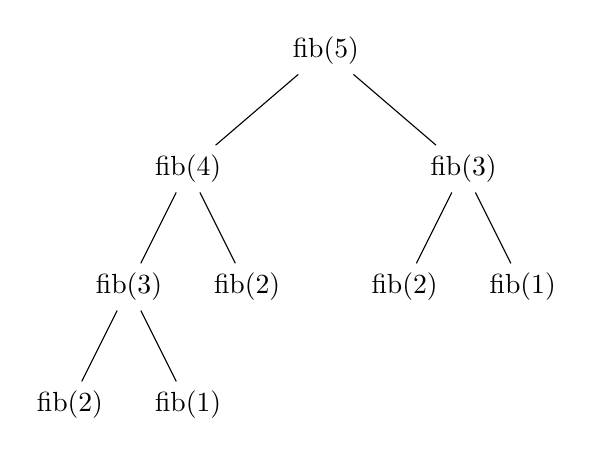
\begin{tikzpicture}
    \node {fib(5)} [sibling distance = 3.5cm]
        child {node {fib(4)} [sibling distance = 1.5cm]
            child {node {fib(3)}
                child {node {fib(2)}}
                child {node {fib(1)}}
            }
            child {node {fib(2)}}
        }
        child {node {fib(3)} [sibling distance = 1.5cm]
            child {node {fib(2)}}
            child {node {fib(1)}}
        };
\end{tikzpicture}
\end{myfigure}

这个程序之所以运行缓慢, 是因为存在大量多余的工作要做, 违反了在\ref{递归}节中叙述的递归的第四条主要法则(合成效益法则). 注意, 在第3行上的第一次调用即$fib(n-1)$实际上在某处计算$fib(n-2)$. 这个信息被抛弃而在第3行上的第二次调用时又重新计算了一遍. 例如在图\ref{斐波那契数列的递归实现中的重复计算}中, $f(3)$被调用了两次, $f(2)$被调用了三次, 如果$N$特别大, 会存在指数级别的重复调用次数. 抛弃的信息量递归地合成起来并导致巨大的运行时间. 这或许是格言``计算任何事情不要超过一次''的最好的实例, 但它不应使你被吓得远离递归而不敢使用. 本课程中将随处看到递归的杰出使用.

\subsection{两数之和{\myleetcode{1}}}

给定一个整数数组\javainline{nums}和一个整数目标值\javainline{target}, 请你在该数组中找出\textbf{和为目标值}\javainline{target}的那\textbf{两个}整数, 并返回它们的数组下标.

你可以假设每种输入只会对应一个答案. 但是, 数组中同一个元素在答案里不能重复出现.

你可以按任意顺序返回答案.

\textbf{示例1}

\begin{mytext}
输入: nums = [2,7,11,15], target = 9
输出: [0,1]
解释: 因为 nums[0] + nums[1] == 9 , 返回 [0, 1] .
\end{mytext}

\textbf{示例2}

\begin{mytext}
输入: nums = [3,2,4], target = 6
输出: [1,2]
\end{mytext}

\textbf{示例3}

\begin{mytext}
输入: nums = [3,3], target = 6
输出: [0,1]
\end{mytext}

\textbf{提示}

\begin{itemize}
    \item $2 \leq nums.length \leq 10^4$
    \item $-10^9 \leq nums[i] \leq 10^9$
    \item $-10^9 \leq target \leq 10^9$
    \item 只会存在一个有效答案
\end{itemize}

\textbf{进阶}: 你可以想出一个时间复杂度小于$O(N^2)$的算法吗?

我们首先考虑的是\textbf{暴力解法}, 也就是将数组中的所有数对都遍历计算一遍, 然后找出符合题意的数对. 代码如程序\ref{两数之和的暴力解法}所示.

\begin{myjava}{label={两数之和的暴力解法}}{两数之和的暴力解法}
public int[] twoSum(int[] nums, int target) {
    for (int i = 0; i < nums.length; i++) { // $N$次循环
        for (int j = i + 1; j < nums.length; j++) { // 最坏情况运行$N-i-1$次循环
            if (nums[i] + nums[j] == target) {
                return new int[]{i, j};
            }
        }
    }
    return new int[]{0,0};
}
\end{myjava}

时间复杂度的分析也比较简单. 最内层循环里面的语句4-6行的时间复杂度是$O(1)$, 那么4-6行会运行多少次呢? 根据以下推导, 可以得知时间复杂度是$O(N^2)$. 空间复杂度的分析也很简单, 我们来看一下程序使用了多少额外空间, 显然我们在程序中只使用了几个局部变量, 所以空间复杂度是$O(1)$.

\begin{equation*}
    \begin{split}
        T(N) &= O(N-1) + O(N-2) + \cdots + O(1) \\
             &= O(N^2)
    \end{split}
\end{equation*}

接下来我们考虑一下能不能使用遍历一次($O(N)$)或者两次($O(2N)=O(N)$)数组就解决问题呢? 因为暴力解法会有两层循环会导致平方级别的时间复杂度.

我们考虑\textbf{缓存}的思想, 也就是先将数组遍历一次, 将数组元素的值和对应的索引保存到哈希表中, 第二次遍历数组时, 直接从哈希表中查找是否存在$target-nums[i]$这个$key$就可以了.

以\textbf{示例1}为例, 第一次遍历$[2,7,11,15]$形成的哈希表:

\begin{tabular}{|c|c|}
    \hline
    \textbf{key(数组元素的值)}  & \textbf{value(数组元素的索引)} \\\hline
    2                & 0                   \\\hline
    7                & 1                   \\\hline
    11               & 2                   \\\hline
    15               & 3                   \\\hline
\end{tabular}

第二次遍历数组, 遍历到元素$2$时, 发现$9-2=7$是哈希表的$key$, 那么直接将$2$的索引和$7$的索引返回即可. 代码如程序\ref{两数之和的两次遍历算法}所示.

\begin{myjava}{label={两数之和的两次遍历算法}}{两数之和的两次遍历算法}
public int[] twoSum(int[] nums, int target) {
    Map<Integer, Integer> map = new HashMap<>();

    // 第1次遍历
    for (int i = 0; i < nums.length; i++) { // $N$次循环
        map.put(nums[i], i); // O(1)
    }

    // 第2次遍历
    for (int i = 0; i < nums.length; i++) {
        Integer anotherIndex = map.get(target - nums[i]); // O(1)
        if (anotherIndex != null && anotherIndex != i) {
            return new int[]{i, anotherIndex};
        }
    }
    return new int[]{0,0};
}
\end{myjava}

在Java中\javainline{HashMap<K, V>}的读写的时间复杂度可以认为是$O(1)$, 我们后面会仔细讨论哈希表的开销. 只有两次循环, 所以时间复杂度是$O(N)$. 由于我们使用了额外的一张哈希表来做缓存, 所以空间复杂度是$O(N)$. 这个例子很好的说明了\textbf{空间换时间}的思想.

我们可以进一步优化上面的程序, 仅遍历一次数组就可以求解问题. 也就是, 我们一边遍历数组元素$nums[i]$, 一边寻找在哈希表中是否存在$target-nums[i]$这个$key$, 如果存在, 直接返回答案. 还是以\textbf{示例1}为例, 遍历完第$0$个元素时, 哈希表如下

\begin{tabular}{|c|c|}
\hline
\textbf{key(数组元素的值)} & \textbf{value(数组元素的索引)} \\\hline
2                        & 0                            \\\hline 
\end{tabular}

在继续遍历$nums[1]=7$时, 发现$9-7=2$已经在哈希表中了, 直接返回索引对$[0,1]$即可.

时间复杂度还是$O(N)$, 只不过优化了常数因子, 空间复杂度还是$O(N)$. 代码如程序\ref{两数之和的一次遍历算法}所示.

\begin{myjava}{label={两数之和的一次遍历算法}}{两数之和的一次遍历算法}
public int[] twoSum(int[] nums, int target) {
    Map<Integer, Integer> map = new HashMap<>();

    for (int i = 0; i < nums.length; i++) {
        Integer anotherIndex = map.get(target - nums[i]);
        if (anotherIndex != null) {
            return new int[]{i, anotherIndex};
        } else {
            map.put(nums[i], i);
        }
    }
    return new int[]{0,0};
}
\end{myjava}

\subsection{三数之和{\myleetcode{15}}}

给你一个整数数组$nums$, 判断是否存在三元组

\begin{equation*}
[nums[i], nums[j], nums[k]]
\end{equation*}

满足$i \neq j, i \neq k \text{且} j \neq k$, 同时还满足

\begin{equation*}
nums[i] + nums[j] + nums[k] \equiv 0
\end{equation*}

请你返回所有和为$0$且不重复的三元组.

注意: 答案中不可以包含重复的三元组.

\textbf{示例1}

\begin{mytext}
输入: nums = [-1,0,1,2,-1,-4]
输出: [[-1,-1,2],[-1,0,1]]
解释: 
nums[0] + nums[1] + nums[2] = (-1) + 0 + 1 = 0 .
nums[1] + nums[2] + nums[4] = 0 + 1 + (-1) = 0 .
nums[0] + nums[3] + nums[4] = (-1) + 2 + (-1) = 0 .
不同的三元组是 [-1,0,1] 和 [-1,-1,2] .
注意, 输出的顺序和三元组的顺序并不重要.
\end{mytext}

\textbf{示例2}

\begin{mytext}
输入: nums = [0,1,1]
输出: []
解释: 唯一可能的三元组和不为 0 .
\end{mytext}

\textbf{示例3}

\begin{mytext}
输入: nums = [0,0,0]
输出: [[0,0,0]]
解释: 唯一可能的三元组和为 0 .
\end{mytext}

\textbf{提示}

\begin{itemize}
    \item $3 \leq nums.length \leq 3000$
    \item $-10^5 \leq nums[i] \leq 10^5$
\end{itemize}

这道题使用\textbf{暴力解法}是可以解决的, 也就是简单的3层循环, 将所有符合条件的三元组都找出来, 然后进行去重. 但这样的问题是时间复杂度太高了$O(N^3)$. 题目中要求找到所有\textbf{不重复}且和为$0$的三元组, 这个\textbf{不重复}的要求使得我们无法简单地使用三重循环枚举所有的三元组. 这是因为在最坏的情况下, 数组中的元素全部为$0$, 即

\begin{mytext}
[0, 0, 0, 0, 0, ..., 0, 0, 0]
\end{mytext}

任意一个三元组的和都为$0$. 如果我们直接使用三重循环枚举三元组, 会得到$O(N^3)$个满足题目要求的三元组(其中$N$是数组的长度)时间复杂度至少为$O(N^3)$. 在这之后, 我们还需要使用哈希表进行去重操作, 得到不包含重复三元组的最终答案, 又消耗了大量的空间. 这个做法的时间复杂度和空间复杂度都很高, 因此我们要换一种思路来考虑这个问题.

我们不管做数学题还是算法题, 首先要做的就是读懂题目的含义, 尽量使用一些\textbf{先验}(预先知道的)的信息, 例如二分查找算法利用的先验信息是: 数组是已经排好序的. 而三数之和题目的先验信息是: 答案不包含重复三元组.

\begin{marker}
例如在大数据开发中, 最重要的一点就是观察和分析数据源的特征. 只有把数据源的各种特性彻底搞明白, 写代码才能得心应手.
\end{marker}

在知道了不重复的先验信息之后, 我们还是采用三层循环的策略. 我们枚举的三元组$(a,b,c)$满足$a\leq b\leq c$, 保证了只有$(a,b,c)$这个顺序会被枚举到, 而$(b,a,c), (c,b,a)$等等这些不会, 这样就减少了重复. 要实现这一点, 我们可以将数组中的元素从小到大进行排序, 随后使用普通的三重循环就可以满足上面的要求.

同时, 对于每一重循环而言, 相邻两次枚举的元素不能相同, 否则也会造成重复. 举个例子, 如果排完序的数组为

\begin{mytext}
[0, 1, 2, 2, 2, 3]
 ^  ^  ^
\end{mytext}

我们使用三重循环枚举到的第一个三元组为$(0,1,2)$, 如果第三重循环继续枚举下一个元素, 那么仍然是三元组$(0,1,2)$, 产生了重复. 因此我们需要将第三重循环``跳到''下一个不相同的元素, 即数组中的最后一个元素$3$, 枚举三元组$(0,1,3)$. 代码如程序\ref{三数之和解法1}所示.

\begin{myjava}{label={三数之和解法1}}{三数之和解法1}
public List<List<Integer>> threeSum(int[] nums) {
    List<List<Integer>> result = new ArrayList<>();

    Arrays.sort(nums);

    for (int i = 0; i < nums.length; i++) {
        if (i > 0 && nums[i] == nums[i - 1]) continue;
        for (int j = i + 1; j < nums.length; j++) {
            if (j > i + 1 && nums[j] == nums[j - 1]) continue;
            for (int k = j + 1; k < nums.length; k++) {
                if (k > j + 1 && nums[k] == nums[k - 1]) continue;
                if (nums[i] + nums[k] + nums[j] != 0) continue;
                List<Integer> cache = new ArrayList<Integer>();
                cache.add(nums[i]);
                cache.add(nums[j]);
                cache.add(nums[k]);
                result.add(cache);
            }
        }
    }

    return result;
}
\end{myjava}

\begin{marker}
解法1在力扣平台运行会超时.
\end{marker}

下面我们来分析一下时间复杂度, 考虑最坏情况, 也就是数组中所有元素都不相等, 且遍历完也没有找到符合要求的三元组. 我们看到有3层循环, 那么我们大概能猜出来时间复杂度是$O(N^3)$, 从代码中可以看出来最费时间的是第11-17行的最内层循环, 这几行代码的执行时间可以化简为$1$个时间单位. 那么最内层循环会执行多少次呢? 精确的分析由和$\sum_{i=0}^{N-1}\sum_{j=i+1}^{N-1}\sum_{k=j+1}^{N-1}1$. 这个和指出了最内层循环执行了多少次. 我们来对这个和进行从内到外的求值.

首先有

\begin{equation*}\begin{split}
\sum_{k=j+1}^{N-1}1 = N - j - 1
\end{split}\end{equation*}

接着可以得到

\begin{equation*}\begin{split}
\sum_{j=i+1}^{N-1}(N-j-1) &= (N-i-2) + (N-i-3) + \cdots + 1 \\
                          &= \frac{(N-i-1)(N-i-2)}{2}
\end{split}\end{equation*}

为了完成全部计算, 我们有

\begin{equation*}\resizebox{1\textwidth}{!}{$\begin{aligned}
\sum_{i=0}^{N-1}\frac{(N-i-1)(N-i-2)}{2} &= \sum_{i=1}^{N}\frac{(N-i)(N-i-1)}{2} \\
&= \frac{1}{2}\sum_{i=1}^{N}i^2 - (N-\frac{1}{2})\sum_{i=1}^{N}i + \frac{1}{2}(N^2-N)\sum_{i=1}^{N}1 \\
&= \frac{1}{2}\frac{N(N+1)(2N+1)}{6} - (N-\frac{1}{2})\frac{N(N+1)}{2} + \frac{1}{2}(N^2-N)N \\
&= \frac{(N-1)(N^2-2)}{6} \\
&= O(N^3)
\end{aligned}$}\end{equation*}

程序中其它代码的时间复杂度, 例如

\begin{itemize}
    \item 第2行: $O(1)$
    \item 第4行: $O(N\log{N})$(排序的时间复杂度)
    \item 第7行: $O(N)$
    \item 第9行: $O(N^2)$
\end{itemize}

相比于$O(N^3)$都可以忽略掉了.

这种方法的时间复杂度仍然为$O(N^3)$, 毕竟我们还是没有跳出三重循环的大框架. 然而它是很容易继续优化的, 可以发现, 如果我们固定了前两重循环枚举到的元素$a$和$b$, 那么只有唯一的$c$满足$a+b+c=0$. 当第二重循环往后枚举一个元素$b'$时, 由于$b'>b$, 那么满足$a+b'+c'=0$的$c'$一定有$c'<c$, 即$c'$在数组中一定出现在$c$的左侧. 也就是说, 我们可以从小到大枚举$b$, 同时从大到小枚举$c$, 即第二重循环和第三重循环实际上是并列的关系.

有了这样的发现, 我们就可以保持第二重循环不变, 而将第三重循环变成一个从数组最右端开始向左移动的指针, 从而得到下面的伪代码:

\subsection{最大子数组和{\myleetcode{53}}}

现在我们将要叙述三个算法来求解早先提出的最大子数组和问题. 第一个算法在程序\ref{最大子数组和的算法1}中表述, 它只是穷举式地尝试所有的可能. for循环中的循环变量反映Java中数组从0开始而不是从1开始这样一个事实.

算法1肯定会正确运行(这不应该花太多时间去证明). 运行时间为$O(N^2)$.

根据代码中的注释, 我们可以计算一下程序的时间复杂度.

\begin{itemize}
    \item 第6行: $O(1)$
    \item 第10行: 由于外层循环运行$N$次, 所以是$O(N)$
    \item 第14-17行: 内存循环中的顺序语句会运行$N + (N-1) + \cdots + 1$次, 而顺序语句的时间复杂度可以由$O(4)$化简成$O(1)$
    \item 第21行: $O(1)$
\end{itemize}

把以上的都加起来, 就可以计算出来时间复杂度了.

\begin{equation*}
    \begin{split}
        T(N) &= O(1) + O(N) + (NO(1) + (N-1)O(1) + \cdots + 1) + O(1) \\
             &= O(1) + O(N) + \sum_{i=1}^{N}O(1) + O(1) \\
             &= O(1) + O(N) + \frac{N(N+1)}{2}O(1) + O(1) \\
             &= O(1) + O(N) + O(\frac{N(N+1)}{2}) + O(1) \\
             &= O(1) + O(N) + O(N^2) + O(1) \\
             &= O(N^2)
    \end{split}
\end{equation*}

\begin{myjava}{label={最大子数组和的算法1}}{求解最大子数组和的算法1}
/**
  * 平方时间的最大子数组和的算法.
  */
public int maxSubArray(int[] nums) {
    // 将最大子数组和初始化为$-\infty$
    int maxSum = Integer.MIN_VALUE; // $O(1)$

    // 两层循环遍历所有可能的子数组.
    for (int i = 0; i < nums.length; i++) { // 循环运行$N$次.
        int thisSum = 0; // $O(1)$
        // 计算$nums[i..j]$这个子数组的和, 如果大于maxSum则更新maxSum.
        // 循环体中的顺序语句的时间复杂度可以简化为$O(1)$.
        for (int j = i; j < nums.length; j++) { // 循环运行$N-i$次.
            thisSum += nums[j]; // $2O(1)=O(1)$, 1次加法操作和1次赋值操作.

            if (thisSum > maxSum) // $O(1)$
                maxSum = thisSum; // $O(1)$
        }
    }

    return maxSum; // $O(1)$
}
\end{myjava}

\begin{marker}
在LeetCode平台运行程序会超时.
\end{marker}

对这个问题有一个递归和相对复杂的$O(N\log{N})$解法, 我们现在就来描述它. 要是真的没出现$O(N)$(线性的)解法, 这个算法就会是体现递归威力的极好的范例了. 该方法采用一种``分治(divide-and-conquer)''策略. 其想法是把问题分成两个大致相等的子问题, 然后递归地对它们求解, 这是``分''的部分. ``治''阶段将两个子问题的解修补到一起并可能再做些少量的附加工作, 最后得到整个问题的解.

在我们的例子中, 最大子序列和可能在三处出现. 或者整个出现在输入数据的左半部, 或者整个出现在右半部, 或者跨越输入数据的中部从而位于左右两半部分之中. 前两种情况可以递归求解. 第三种情况的最大和可以通过求出前半部分(包含前半部分最后一个元素)的最大和以及后半部分(包含后半部分第一个元素)的最大和而得到. 此时将这两个和相加. 作为一个例子, 考虑下列输入:

\begin{tabular}{|cccc|cccc|}
    \hline
    \multicolumn{4}{|c|}{前半部分} & \multicolumn{4}{|c|}{后半部分} \\
    \hline
    4 & -3 & 5 & -2 & -1 & 2 & 6 & -2 \\
    \hline
\end{tabular}

其中前半部分的最大子序列和为6(从元素$A_1$到$A_3$)而后半部分的最大子序列和为8(从元素$A_6$到$A_7$).

前半部分包含其最后一个元素的最大和是4(从元素$A_1$到$A_4$), 而后半部分包含其第一个元素的最大和是7(从元素$A_5$到$A_7$). 因此, 横跨这两部分且通过中间的最大和为4+7=11(从元素$A_1$到$A_7$).

我们看到, 在形成本例中的最大和子序列的三种方式中, 最好的方式是包含两部分的元素. 于是, 答案为11. 程序\ref{最大子数组和的算法2}提出了这种策略的一种实现手段.

有必要对算法2的程序进行一些说明. 递归过程调用的一般形式是传递输入的数组以及左边界和右边界, 它们界定了数组要被处理的部分. 单行驱动程序通过传递数组以及边界$0$和$N-1$而将该过程启动.

第8行至第12行处理基准情况. 如果\javainline{left == right}, 那么只有一个元素, 并且当该元素非负时它就是最大子序列. \javainline{left > right}的情况是不可能出现的, 除非$N$是负数(不过, 程序中小的扰动有可能致使这种混乱产生). 第15行和第16行执行两个递归调用. 我们可以看到, 递归调用总是对小于原问题的问题进行, 不过程序中的小扰动有可能破坏这个特性. 第18行至第24行以及第26行至第32行计算达到中间分界处的两个最大和的和数. 这两个值的和为扩展到左右两部分的最大和. 程序\javainline{max3}返回这三个可能的最大和中的最大者.

显然, 算法2需要比算法1更多的编程努力. 然而, 程序短并不总意味着程序好. 正如我们在前面显示算法运行时间的表中已经看到的, 除最小的输入量外, 算法2比算法1明显要快.

对运行时间的分析方法与在分析计算斐波那契数程序时的方法类似. 令$T(N)$是求解大小为$N$的最大子序列和问题所花费的时间. 如果$N=1$, 则算法3执行程序第8行到第12行花费某个常数时间量, 我们称之为一个时间单位. 于是, $T(1)=O(1)$. 否则, 程序必须运行两个递归调用, 即在第19行和第32行之间的两个for循环, 以及某个小的簿记量, 如第14行和第18行. 这两个for循环总共接触到从$A_0$到$A_{N-1}$的每一个元素, 而在循环内部的工作量是常量, 因此, 在第19到32行花费的时间为$O(N)$. 在第8行到第14行, 第18, 26和34行上的程序的工作量都是常量, 从而与$O(N)$相比可以忽略. 其余就是第15, 16行上运行的工作. 这两行求解大小为$N/2$的子序列问题(假设$N$是偶数). 因此, 这两行每行花费$T(N/2)$个时间单元, 共花费$2T(N/2)$个时间单元. 算法3花费的总的时间为$2T(N/2)+O(N)$. 我们得到方程组

\begin{equation*}
    \begin{split}
        T(1) &= O(1) \\
        T(N) &= 2T(N/2)+O(N)
    \end{split}
\end{equation*}

\begin{myjava}{label={最大子数组和的算法2}}{求解最大子数组和的算法2}
/**
 * 返回三个int数值中的最大值.
 */
private int max3(int num1, int num2, int num3) {
    int max = num1; // 假设第一个数为最大值

    // 比较第二个数和第三个数, 更新最大值
    if (num2 > max) {
        max = num2;
    }
    if (num3 > max) {
        max = num3;
    }

    return max; // 返回最大值
}

/**
 * 最大子数组和的递归算法.
 * 寻找a[left..right]范围的最大子数组和.
 */
private int maxSumRec(int[] a, int left, int right) {
    if (left == right) // 基准情形
        return a[left];

    int center = (left + right) / 2;
    int maxLeftSum = maxSumRec(a, left, center);
    int maxRightSum = maxSumRec(a, center + 1, right);

    int maxLeftBorderSum = Integer.MIN_VALUE, leftBorderSum = 0;
    for (int i = center; i >= left; i--) {
        leftBorderSum += a[i];
        if (leftBorderSum > maxLeftBorderSum)
            maxLeftBorderSum = leftBorderSum;
    }

    int maxRightBorderSum = Integer.MIN_VALUE, rightBorderSum = 0;
    for (int i = center + 1; i <= right; i++) {
        rightBorderSum += a[i];
        if (rightBorderSum > maxRightBorderSum)
            maxRightBorderSum = rightBorderSum;
    }

    return max3(maxLeftSum, maxRightSum,
                maxLeftBorderSum + maxRightBorderSum);
}

/**
 * 最大子数组和的分治算法的程序驱动器
 */
public int maxSubArray(int[] nums) {
    return maxSumRec(nums, 0, nums.length - 1);
}
\end{myjava}

接下来我们介绍求解最大子序列和的第3种方法, 该算法实现起来要比递归算法简单而且更为有效. 在程序\ref{最大子数组和的算法3}中给出.

\begin{myjava}{label={最大子数组和的算法3}}{求解最大子数组和的算法3}
/**
 * 线性时间复杂度的最大子序列和算法.
 */
public int maxSubArray(int[] nums) {
    int thisSum = 0, maxSum = nums[0];
    for (int x : nums) {
        thisSum = Math.max(thisSum + x, x);
        maxSum = Math.max(maxSum, thisSum);
    }
    return maxSum;
}
\end{myjava}

不难理解为什么时间的界是正确的, 但是要明白为什么算法是正确可行的却需要多加思考.

假设$nums$数组的长度是$N$, 下标从$0$到$N-1$.

我们用$f(i)$代表以第$i$个数结尾的``连续子数组的最大和'', 那么很显然我们要求的答案就是:

\begin{equation*}
    \max_{0\leq i \leq N-1}{f(i)}
\end{equation*}

因此我们只需要求出每个位置的$f(i)$, 然后返回$f$数组中的最大值即可. 那么我们如何求$f(i)$呢? 我们可以考虑$nums[i]$单独成为一段还是加入$f(i-1)$对应的那一段, 这取决于$nums[i]$和$f(i-1)+nums[i]$的大小, 我们希望获得一个比较大的, 于是可以写出这样的动态规划转移方程:

\begin{equation*}
    f(i) = \max{(f(i-1)+nums[i],nums[i])}
\end{equation*}

不难给出一个时间复杂度$O(N)$, 空间复杂度$O(N)$的实现, 即用一个$f$数组来保存$f(i)$的值, 用一个循环求出所有$f(i)$. 考虑到$f(i)$只和$f(i-1)$相关, 于是我们可以只用一个变量$thisSum$来维护对于当前$f(i)$的$f(i-1)$的值是多少, 从而让空间复杂度降低到$O(1)$, 这有点类似``滚动数组''的思想.

这个算法是许多聪明算法的典型: 运行时间是明显的, 但正确性则不那么容易看出来. 对于这些算法, 正式的正确性证明(比上面的分析更正式)几乎总是需要的; 然而, 即使到那时, 许多人仍然还是不信服. 此外, 许多这类算法需要更有技巧的编程, 这导致更长的开发过程. 不过当这些算法正常工作时, 它们运行得很快, 而我们将它们和一个低效(但容易实现)的蛮力算法通过小规模的输入进行比较可以测试到大部分的程序原理.

该算法的一个附带的优点是, 它只对数据进行一次扫描, 一旦$nums[i]$被读入并被处理, 它就不再需要被记忆. 因此, 如果数组在磁盘上或通过互联网传送, 那么它就可以被按顺序读入, 在主存中不必存储数组的任何部分. 不仅如此, 在任意时刻, 算法都能对它已经读入的数组给出子序列问题的正确答案(其它算法不具有这个特性). 具有这种特性的算法叫做\textbf{在线算法}(online algorithm). 仅需要常量空间并以线性时间运行的在线算法几乎是完美的算法.

\subsection{运行时间中的对数}

分析算法最混乱的方面大概集中在对数上面. 我们已经看到, 某些分治算法将以$O(N\log{N})$时间运行. 此外, 对数最常出现的规律可概括为下列一般法则: 如果一个算法用常数时间($O(1)$)将问题的大小削减为其一部分(通常是$1/2$), 那么该算法就是$O(\log{N})$. 另一方面, 如果使用常数时间只是把问题减少一个常数的数量(如将问题减少$1$), 那么这种算法就是$O(N)$的.

显然, 只有一些特殊种类的问题才能够呈$O(\log{N})$型. 例如, 若输入$N$个数, 则算法只要把这些数读入就必须耗费$O(N)$的时间量. 因此, 当我们谈到这类问题的$O(\log{N})$算法时, 通常都是假设输入数据已经提前读入. 下面, 我们提供具有对数特点的三个例子.

\subsubsection{二分查找}

第一个例子通常叫作二分查找(binary search).

二分查找: 给定一个整数$X$和整数$A_0, A_1, \cdots, A_{N-1}$, 后者已经预先排序并在内存中, 求下标$i$使得$A_i=X$, 如果$X$不在数据中, 则返回$i=-1$.

明显的解法是从左到右扫描数据, 其运行花费线性时间. 然而, 这个算法没有用到该列表已经排序的事实, 这就使得算法很可能不是最好的. 一个好的策略是验证$X$是否是居中的元素. 如果是, 则答案就找到了. 如果$X$小于居中元素, 那么我们可以应用同样的策略于居中元素左边已排序的子序列; 同理, 如果$X$大于居中元素, 那么我们检查数据的右半部分. (同样, 也存在可能会终止的情况.)程序\ref{二分查找算法}列出了二分查找的程序(其答案为$mid$). 图中的程序同样也反映了Java语言数组下标从0开始的惯例.

\begin{myjava}{label={二分查找算法}}{二分查找算法}
public static binarySearch(int[] a, int x) {
    int low = 0, high = a.length - 1;

    while (low <= high) {
        int mid = (low + high) / 2;

        if (a[mid] < x) {
            low = mid + 1;
        } else if (a[mid] > x) {
            high = mid - 1;
        } else {
            return mid;
        }
    }

    return -1;
}
\end{myjava}

显然, 每次迭代在循环内的所有工作花费$O(1)$, 因此分析需要确定循环的次数. 循环从$high-low=N-1$开始, 并保持$high-low\geq 1$. 每次循环后$high-low$的值至少将该次循环前的值折半; 于是, 循环的次数最多为$\lceil log(N-1)\rceil +2$.(例如, 若$high-low=128$, 则在各次迭代后$high-low$的最大值是64, 32, 16, 8, 4, 2, 1.0, -1.) 因此, 运行时间是$O(\log{N})$. 与此等价, 我们也可以写出运行时间的递推公式, 不过, 当我们理解实际在做什么以及为什么的原理时, 这种强行写公式的做法通常没有必要.

二分查找可以看作是我们的第一个数据结构实现方法, 它提供了在$O(\log{N})$时间内的\javainline{contains}操作, 但是所有其他操作(特别是\javainline{insert}操作)均需要$O(N)$时间. 在数据是稳定(即不允许插入操作和删除操作)的应用中, 这种操作可能是非常有用的. 此时输入数据需要一次排序, 但是此后的访问会很快.

\subsubsection{搜索旋转排序数组\myleetcode{33}}

\subsubsection{搜索二维矩阵II\myleetcode{240}}

\subsubsection{寻找两个正序数组的中位数\myleetcode{4}}

\subsubsection{欧几里得算法}

\begin{myjava}{label={欧几里得算法}}{欧几里得算法}
public static long gcd(long m, long n) {
    while (n != 0) {
        long rem = m % n;
        m = n;
        n = rem;
    }

    return m;
}
\end{myjava}

第二个例子是计算最大公因数的欧几里得算法. 两个整数的最大公因数(gcd)是同时整除二者的最大整数. 于是, $gcd(50,15)=5$. 程序\ref{欧几里得算法}所示的算法计算$gcd(M,N)$, 假设$M\geq N$(如果$N>M$, 则循环的第一次迭代将它们互相交换).

算法连续计算余数直到余数是0为止, 最后的非零余数就是最大公因数. 因此, 如果$M=1989$和$N=1590$, 则余数序列是399, 393, 6, 3, 0. 从而, $gcd(1989, 1590)=3$. 正如例	子所表明的, 这是一个快速算法.

如前所述, 估计算法的整个运行时间依赖于确定余数序列究竟有多长. 虽然$\log{N}$看似像理想中的答案, 但是根本看不出余数的值按照常数因子递减的必然性, 因为我们看到, 例中的余数从399仅仅降到393. 事实上, 在一次迭代中余数并不按照一个常数因子递减. 然而, 我们可以证明, 在两次迭代以后, 余数最多是原始值的一半. 这就证明了, 迭代次数至多是$2\log{N}=O(\log{N})$从而得到运行时间. 这个证明并不难, 因此我们将它放在这里, 可从下列定理直接推出它.

\begin{mytheorem}{}{}
如果$M>N$, 则$M\mod{N}<M/2$.
\end{mytheorem}

\begin{myproof}{}{}
存在两种情形. 如果$N\leq M/2$, 则由于余数小于$N$, 故定理在这种情形下成立. 另一种情形是$N>M/2$. 但是此时$M$仅含有一个$N$从而余数为$M-N<M/2$, 定理得证.
\end{myproof}

从上面的例子来看, $2\log{N}$大约为$20$, 而我们仅进行了$7$次运算, 因此有人会怀疑这是不是可能的最好的界. 事实上, 这个常数在最坏的情况下还可以稍微改进成$1.44\log{N}$(如$M$和$N$是两个相邻的斐波那契数时就是这种情况). 欧几里得算法在平均情况下的性能需要大量篇幅的高度复杂的数学分析, 其迭代的平均次数约为$(12\ln{2}\ln{N})/\pi+1.47$.

\textbf{幂运算}

\begin{myjava}{label={高效率的幂运算}}{高效率的幂运算}
public static long pow(long x, int n) {
    if (n == 0) return 1;
    if (n == 1) return x;
    if (n % 2 == 0) {
        return pow(x * x, n / 2);
    } else {
        return pow(x * x, n / 2) * x;    
    }
}
\end{myjava}

我们在本节的最后一个例子是处理一个整数的幂(它还是一个整数). 由取幂运算得到的数一般都是相当大的, 因此, 我们只能在假设有一台机器能够存储这样一些大整数(或有一个编译程序能够模拟它)的情况下进行我们的分析. 我们将用乘法的次数作为运行时间的度量.

计算$X^N$的明显的算法是使用$N-1$次乘法自乘. 有一种递归算法效果更好. $N\leq 1$是这种递归的基准情形. 否则, 若$N$是偶数, 我们有$X^N=X^{N/2}\cdot X^{N/2}$, 如果$N$是奇数, 则$X=X^{(N-1)/2}\cdot X^{(N-1)/2}\cdot X$.

例如, 为了计算$X^62$, 算法将如下进行, 它只用到$9$次乘法:

\begin{equation*}
    X^3=(X^2)X, X^7=(X^3)^2X, X^{15}=(X^7)^2X, X^{31}=(X^{15})^2X, X^{62}=(X^{31})^2
\end{equation*}

显然, 所需要的乘法次数最多是$2\log{N}$, 因为把问题分半最多需要两次乘法(如果$N$是奇数). 这里, 我们又可写出一个递推公式并将其解出. 简单的直觉避免了盲目的强行处理.

程序\ref{高效率的幂运算}中的代码实现了这个想法. 有时候看一看程序能够进行多大的调整而不影响其正确性倒是很有意思的. 在程序\ref{高效率的幂运算}中, 第5行到第6行实际上不是必需的, 因为如果$N$是$1$, 那么第10行将做同样的事情. 第10行还可以写成:

\javainline{return pow(x, n - 1) * x;}

而不影响程序的正确性. 事实上, 程序仍将以$O(\log{n})$运行, 因为乘法的序列同以前一样. 不过, 下面所有对第8行的修改都是不可取的, 虽然它们看起来似乎都正确:

\begin{enumerate}
    \item \javainline{return pow(pow(x, 2), n / 2);}
    \item \javainline{return pow(pow(x, n / 2), 2);}
    \item \javainline{return pow(x, n / 2) * pow(x, n / 2);}
\end{enumerate}

1和2两行都是不正确的, 因为当$N$是2时递归调用pow中有一个是以2作为第2个参数. 这样, 程序产生一个无限循环, 将不能往下进行(最终导致程序非正常终止).

使用第3行会影响程序的效率, 因为此时有两个大小为$N/2$的递归调用而不是一个. 分析指出, 其运行时间不再是$O(\log{N})$.

\subsection{分析结果的准确性}

根据经验, 有时分析会估计过大. 如果这种情况发生, 那么或者需要进一步细化分析(一般通过机敏的观察), 或者可能是平均运行时间显著小于最坏情形的运行时间, 不可能对所得的界再加以改进. 对于许多复杂的算法, 最坏的界通过某个坏的输入是可以达到的, 但在实践中它通常是估计过大的. 遗憾的是, 对于大多数这类问题, 平均情形的分析是极其复杂的(在许多情形下仍然悬而未决), 而最坏情形的界尽管过分地悲观, 但却是最好的已知解析结果.

\chapter{表, 栈和队列}

本章讨论最简单和最基本的三种数据结构. 实际上, 每一个有意义的程序都将显式地至少使用一种这样的数据结构, 而栈则在程序中总是要被间接地用到, 不管我们在程序中是否做了声明. 本章重点是:

\begin{itemize}
  \item 介绍抽象数据类型的概念.
  \item 阐述如何有效地执行表的操作.
  \item 介绍栈ADT及其在实现递归方面的应用.
  \item 介绍队列ADT及其在操作系统和算法设计中的应用.
\end{itemize}

在这一章, 我们提供实现两个库类重要子集\javainline{ArrayList}和\javainline{LinkedList}的代码.

\section{抽象数据类型}

抽象数据类型(abstract data type, ADT)是带有一组操作的一些对象的集合. 抽象数据类型是数学的抽象; 在ADT的定义中没有地方提到关于这组操作是如何实现的任何解释. 诸如表, 集合, 图以及与它们各自的操作一起形成的这些对象都可以被看做是抽象数据类型, 这就像整数, 实数, 布尔数都是数据类型一样. 整数, 实数和布尔数各自都有与之相关的操作, 而抽象数据类型也是如此. 对于集合ADT, 可以有像添加(add), 删除(remove)以及包含(contain)这样一些操作. 当然, 也可以只要两种操作并(union)和查找(find), 这两种操作又在这个集合上定义了一种不同的ADT.

Java类也考虑到ADT的实现, 不过适当地隐藏了实现的细节. 这样, 程序中需要对ADT实施操作的任何其他部分可以通过调用适当的方法来进行. 如果由于某种原因需要改变实现的细节, 那么通过仅仅改变执行这些ADT操作的例程应该是很容易做到的. 这种改变对于程序的其余部分是完全透明的.

对于每种ADT并不存在什么法则来告诉我们必须要有哪些操作, 这是一个设计决策. 错误处理和结构调整(在适当的地方)一般也取决于程序的设计者. 本章中将要讨论的这三种数据结构是ADT的最基本的例子. 我们将会看到它们中的每一种是如何以多种方法实现的, 不过, 当它们被正确地实现以后,使用它们的程序却没有必要知道它们是如何实现的.

\subsection{表ADT}

我们将处理形如$A_0,A_1,A_2,\cdots,A_{N-1}$的一般的表. 我们说这个表的大小是$N$. 我们将大小为$O$的特殊的表称为\textbf{空表}(empty list).

对于除空表外的任何表, 我们说$A_i$后继$A_{i-1}$(或继$A_{i-1}$之后, $i<N$)并称$A_{i-1}$前驱$A_i(i>0)$.

表中的第一个元素是$A_0$, 而最后一个元素是$A_{N-1}$. 我们将不定义$A_0$的前驱元, 也不定义$A_{N-1}$的后继元. 元素$A_i$在表中的位置为$i+1$. 为了简单起见, 我们假设表中的元素是整数, 但一般说来任意的复元素也是允许的(而且容易由Java泛型类处理).

与这些``定义''相关的是要在表ADT上进行操作的集合.

\javainline{printList}和\javainline{makeEmpty}是常用的操作, 其功能显而易见; \javainline{find}返回某一项首次出现的位置; \javainline{insert}和 \javainline{remove}一般是从表的某个位置插入和删除某个元素; 而\javainline{findKth}则返回(作为参数而被指定的)某个位置上的元素. 如果$34,12,52,16,12$是一个表, 则\javainline{find(52)}会返回$2$; \javainline{insert(x,2)}可把表变成$34,12,x,52,16,12$(如果我们插入到给定位置上的话); 而\javainline{remove(52)}则又将该表变为$34,12,x,16,12$.

当然, 一个方法的功能怎样才算恰当, 完全要由程序设计者来确定, 就像对特殊情况的处理那样(例如, 上述\javainline{find(1)}返回什么?). 我们还可以添加一些操作, 比如\javainline{next}和\javainline{previous}, 它们会取一个位置作为参数并分别返回其后继元和前驱元的位置.

\subsection{表的简单数组实现}

对表的所有这些操作都可以通过使用数组来实现. 虽然数组是由固定容量创建的, 但在需要的时候可以用双倍的容量创建一个不同的数组. 它解决由于使用数组而产生的最严重的问题, 即从历史上看为了使用一个数组, 需要对表的大小进行估计. 而这种估计在Java或任何现代编程语言中都是不需要的. 下列程序段解释一个数组\javainline{arr}在必要的时候如何被扩展(其初始长度为$10$):

\begin{myjava}{}{}
int[] arr = new int[10];

// 下面我们决定需要扩大arr.
int[] newArr = new int[arr.length * 2];

for(int i = O; i < arr.length; i++)
    newArr[i] = arr[i];
arr newArr;
\end{myjava}

数组的实现可以使得\javainline{printList}以线性时间被执行, 而\javainline{findKth}操作则花费常数时间, 这正是我们所能够预期的. 不过, 插入和删除的花费却潜藏着昂贵的开销, 这要看插入和删除发生在什么地方. 最坏的情形下, 在位置$0$的插入(即在表的前端插入)首先需要将整个数组后移一个位置以空出空间来, 而删除第一个元素则需要将表中的所有元素前移一个位置, 因此这两种操作的最坏情况为$O(N)$. 平均来看, 这两种操作都需要移动表的一半的元素, 因此仍然需要线性时间. 另一方面, 如果所有的操作都发生在表的高端, 那就没有元素需要移动, 而添加和删除则只花费$O(1)$时间.

存在许多情形, 在这些情形下的表是通过在高端进行插入操作建成的, 其后只发生对数组的访问(即只有\javainline{findKth}操作). 在这种情况下, 数组是表的一种恰当的实现. 然而, 如果发生对表的一些插入和删除操作, 特别是对表的前端进行, 那么数组就不是一种好的选择. 下一节处理另一种数据结构: \textit{链表}(linked list).

\subsection{简单链表}

为了避免插入和删除的线性开销, 我们需要保证表可以不连续存储, 否则表的每个部分都可能需要整体移动. 图\ref{一个链表}指出链表的一般想法.

\begin{myfigure}[label={一个链表}]{一个链表}\scalebox{.6}{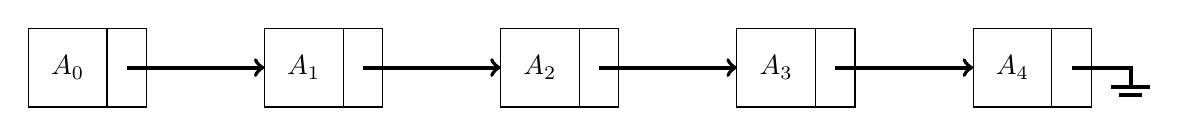
\begin{tikzpicture}
\draw (0,0) rectangle (1,1) node[pos=.5] {$A_0$};
\draw (1,0) rectangle (1.5,1) node[pos=.5] {};

\draw (3,0) rectangle (4,1) node[pos=.5] {$A_1$};
\draw (4,0) rectangle (4.5,1) node[pos=.5] {};

\draw (6,0) rectangle (7,1) node[pos=.5] {$A_2$};
\draw (7,0) rectangle (7.5,1) node[pos=.5] {};

\draw (9,0) rectangle (10,1) node[pos=.5] {$A_3$};
\draw (10,0) rectangle (10.5,1) node[pos=.5] {};

\draw (12,0) rectangle (13,1) node[pos=.5] {$A_4$};
\draw (13,0) rectangle (13.5,1) node[pos=.5] {};

\draw [->, line width=0.5mm] (1.25,0.5) -- (3,0.5);
\draw [->, line width=0.5mm] (4.25,0.5) -- (6,0.5);
\draw [->, line width=0.5mm] (7.25,0.5) -- (9,0.5);
\draw [->, line width=0.5mm] (10.25,0.5) -- (12,0.5);
\draw [-, line width=0.5mm] (13.25,0.5) -- (14,0.5) -- (14,0.25);

\draw [-, line width=0.5mm] (13.75,0.25) -- (14.25,0.25);
\draw [-, line width=0.5mm] (13.85,0.15) -- (14.15,0.15);
\end{tikzpicture}}\end{myfigure}

链表由一系列节点组成, 这些节点不必在内存中相连. 每一个节点均含有表元素和到包含该元素后继元的节点的链(link). 我们称之为\javainline{next}链. 最后一个单元的\javainline{next}链引用\javainline{null}.

为了执行\javainline{printList}或\javainline{find(x)}, 只要从表的第一个节点开始然后用一些后继的\javainline{next}链遍历该表即可. 这种操作显然是线性时间的, 和在数组实现时一样, 不过其中的常数可能会比用数组实现时要大. \javainline{findKth}操作不如数组实现时的效率高; \javainline{findKth(i)}花费$O(i)$的时
间并以这种明显的方式遍历链表而完成. 在实践中这个界是保守的, 因为调用\javainline{findKth}常常是以($按i$)排序后的方式进行. 例如, \javainline{findKth(2)}, \javainline{findKth(3)}, \javainline{findKth(4)}以及\javainline{findKth(6)}可通过对表的一次扫描同时实现.

\javainline{remove}方法可以通过修改一个\javainline{next}引用来实现. 图\ref{从链表中删除}给出在原表中删除第三个元素的结果.

\begin{myfigure}[label={从链表中删除}]{从链表中删除}\scalebox{.6}{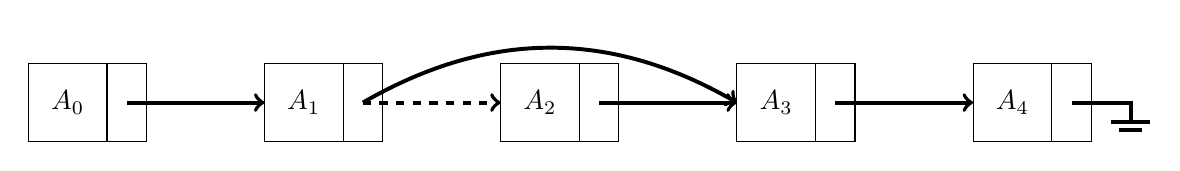
\begin{tikzpicture}
\draw (0,0) rectangle (1,1) node[pos=.5] {$A_0$};
\draw (1,0) rectangle (1.5,1) node[pos=.5] {};

\draw (3,0) rectangle (4,1) node[pos=.5] {$A_1$};
\draw (4,0) rectangle (4.5,1) node[pos=.5] {};

\draw (6,0) rectangle (7,1) node[pos=.5] {$A_2$};
\draw (7,0) rectangle (7.5,1) node[pos=.5] {};

\draw (9,0) rectangle (10,1) node[pos=.5] {$A_3$};
\draw (10,0) rectangle (10.5,1) node[pos=.5] {};

\draw (12,0) rectangle (13,1) node[pos=.5] {$A_4$};
\draw (13,0) rectangle (13.5,1) node[pos=.5] {};

\draw [->, line width=0.5mm] (1.25,0.5) -- (3,0.5);
\draw [->, line width=0.5mm, dashed] (4.25,0.5) -- (6,0.5);
\draw [->, line width=0.5mm] (7.25,0.5) -- (9,0.5);
\draw [->, line width=0.5mm] (10.25,0.5) -- (12,0.5);
\draw [-, line width=0.5mm] (13.25,0.5) -- (14,0.5) -- (14,0.25);
\draw [->, line width=0.5mm] (4.25,0.5) to[out=30,in=150] (9,0.5);

\draw [-, line width=0.5mm] (13.75,0.25) -- (14.25,0.25);
\draw [-, line width=0.5mm] (13.85,0.15) -- (14.15,0.15);
\end{tikzpicture}}\end{myfigure}

\javainline{insert}方法需要使用\javainline{new}操作符从系统取得一个新节点, 此后执行两次引用的调整. 其一般想法在图\ref{向链表查入}中给出, 其中的虚线表示原来的\javainline{next}引用.

\begin{myfigure}[label={向链表插入}]{向链表插入}\scalebox{.6}{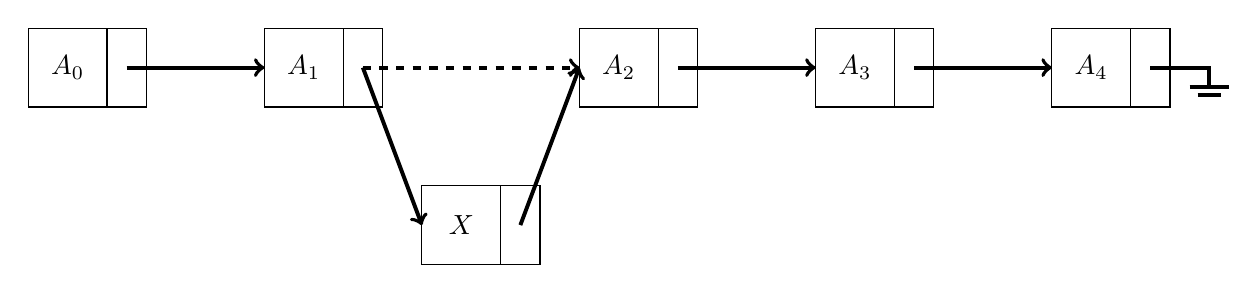
\begin{tikzpicture}
\draw (0,0) rectangle (1,1) node[pos=.5] {$A_0$};
\draw (1,0) rectangle (1.5,1) node[pos=.5] {};

\draw (3,0) rectangle (4,1) node[pos=.5] {$A_1$};
\draw (4,0) rectangle (4.5,1) node[pos=.5] {};

\draw (5,-2) rectangle (6,  -1) node[pos=.5] {$X$};
\draw (6,-2) rectangle (6.5,-1) node[pos=.5] {};

\draw (7,0) rectangle (8,1) node[pos=.5] {$A_2$};
\draw (8,0) rectangle (8.5,1) node[pos=.5] {};

\draw (10,0) rectangle (11,1) node[pos=.5] {$A_3$};
\draw (11,0) rectangle (11.5,1) node[pos=.5] {};

\draw (13,0) rectangle (14,1) node[pos=.5] {$A_4$};
\draw (14,0) rectangle (14.5,1) node[pos=.5] {};

\draw [->, line width=0.5mm] (1.25,0.5) -- (3,0.5);
\draw [->, line width=0.5mm,dashed] (4.25,0.5) -- (7,0.5);
\draw [->, line width=0.5mm] (8.25,0.5) -- (10,0.5);
\draw [->, line width=0.5mm] (11.25,0.5) -- (13,0.5);
\draw [-, line width=0.5mm] (14.25,0.5) -- (15,0.5) -- (15,0.25);

\draw [-, line width=0.5mm] (14.75,0.25) -- (15.25,0.25);
\draw [-, line width=0.5mm] (14.85,0.15) -- (15.15,0.15);

\draw [->, line width=0.5mm] (4.25,0.5) -- (5,-1.5);
\draw [->, line width=0.5mm] (6.25, -1.5) -- (7,0.5);
\end{tikzpicture}}\end{myfigure}

我们看到, 在实践中如果知道变动将要发生的地方, 那么向链表插入或从链表中删除一项的操作不需要移动很多的项, 而只涉及常数个节点链的改变.

在表的前端添加项或删除第一项的特殊情形此时也属于常数时间的操作, 当然要假设到链表前端的链是存在的. 只要我们拥有到链表最后节点的链, 那么在链表末尾进行添加操作的特殊情形(即让新的项成为最后一项)可以花费常数时间. 因此, 典型的链表拥有到该表两端的链. 删除最后一项比较复杂, 因为必须找出指向最后节点的项, 把它的\javainline{next}链改成\javainline{null}, 然后再更新持有最后节点的链. 在经典的链表中, 每个节点均存储到其下一节点的链, 而拥有指向最后节点的链并不提供最后节点的前驱节点的任何信息.

保留指向最后节点的节点的第3个链的想法行不通, 因为它在删除操作期间也需要更新. 我们的做法是, 让每一个节点持有一个指向它在表中的前驱节点的链, 如图\ref{双向链表}所示, 我们称之为双向链表(doubly linked list).

\begin{myfigure}[label={双向链表}]{双向链表}\scalebox{.6}{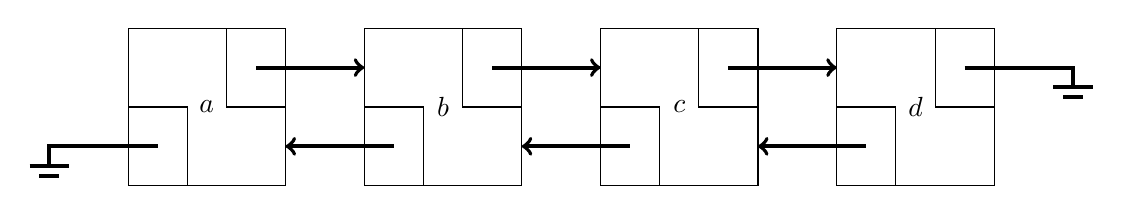
\begin{tikzpicture}
\draw (0,0) rectangle (2,2) node[pos=.5] {$a$};
\draw (1.25,1) rectangle (2,2) node[pos=.5] {};
\draw (0,0) rectangle (0.75,1) node[pos=.5] {};

\draw (3,0) rectangle (5,2) node[pos=.5] {$b$};
\draw (4.25,1) rectangle (5,2) node[pos=.5] {};
\draw (3,0) rectangle (3.75,1) node[pos=.5] {};

\draw (6,0) rectangle (8,2) node[pos=.5] {$c$};
\draw (7.25,1) rectangle (8,2) node[pos=.5] {};
\draw (6,0) rectangle (6.75,1) node[pos=.5] {};

\draw (9,0) rectangle (11,2) node[pos=.5] {$d$};
\draw (10.25,1) rectangle (11,2) node[pos=.5] {};
\draw (9,0) rectangle (9.75,1) node[pos=.5] {};

\draw [->, line width=0.5mm] (1.625,1.5) -- (3,1.5);
\draw [->, line width=0.5mm] (4.625,1.5) -- (6,1.5);
\draw [->, line width=0.5mm] (7.625,1.5) -- (9,1.5);

\draw [<-, line width=0.5mm] (2,0.5) -- (3.375,0.5);
\draw [<-, line width=0.5mm] (5,0.5) -- (6.375,0.5);
\draw [<-, line width=0.5mm] (8,0.5) -- (9.375,0.5);

\draw [-, line width=0.5mm] (0.375,0.5) -- (-1,0.5) -- (-1, 0.25);
\draw [-, line width=0.5mm] (-1.25,0.25) -- (-0.75,0.25);
\draw [-, line width=0.5mm] (-1.125,0.125) -- (-0.875,0.125);

\draw [-, line width=0.5mm] (10.625,1.5) -- (12,1.5) -- (12,1.25);
\draw [-, line width=0.5mm] (11.75,1.25) -- (12.25,1.25);
\draw [-, line width=0.5mm] (11.875,1.125) -- (12.125,1.125);
\end{tikzpicture}}\end{myfigure}

\section{Java Collections API中的表}

在类库中, Java语言包含有一些普通数据结构的实现. 该语言的这一部分通常叫作Collections API. 表ADT是在Collections API中实现的数据结构之一. 我们将在第4章看到其他一些数据结构.

\subsection{Collection接口}

Collections API位于java.util包中. 集合(collection)的概念在Collection接口中得到抽象, 它存储一组类型相同的对象. 程序\ref{java.util包中Collection接口的子集}显示该接口一些最重要的部分(但一些方法未被显示).

在Collection接口中的许多方法所做的工作由它们的英文名称可以看出, 因此size返回集合中的项数; isEmpty返回true当且仅当集合的大小为O. 如果x在集合中, 则contains返回true. 注意, 这个接口并不规定集合如何决定x是否属于该集合--这要由实现该Collection接口的具体的类来确定. add和remove从集合中添加和删除x, 如果操作成功则返回true, 如果因某个看似有理(非异常)的原因失败则返回false. 例如, 如果要删除的项不在集合中, 则remove可能失败, 而如果特定的集合不允许重复, 那么当企图插入一项重复项时, add操作就可能失败.

\begin{myjava}{label={java.util包中Collection接口的子集}}{java.util包中Collection接口的子集}
public interface Collection<T> {
    int size();
    boolean isEmpty();
    void clear();
    boolean contains(T x);
    boolean add(T x);
    boolean remove(T x);
}
\end{myjava}

\subsection{List接口, ArrayList类和LinkedList类}

本节跟我们关系最大的集合就是表(list), 它由java.util包中的List接口指定. List接口继承了Collection接口, 因此它包含Collection接口的所有方法, 外加其他一些方法. 代码\ref{java.util包中List接口的子集}解释其中最重要的一些方法.

\begin{myjava}{label={java.util包中List接口的子集}}{java.util包中List接口的子集}
public interface List<T> extends Collection<T> {
    T get(int idx);
    T set(int idx, T newVal);
    void add(int idx, T x);
    void remove(int idx);
}
\end{myjava}

get和set使得用户可以访问或改变通过由位置索引idx给定的表中指定位置上的项. 索引O位于表的前端, 索引size()-1代表表中的最后一项, 而索引size()则表示新添加的项可以被放置的位置. add使得在位置idx处置入一个新的项(并把其后的项向后推移一个位置). 于是, 在位置O处add是在表的前端进行的添加, 而在位置size()处的add是把被添加项作为新的最后项添入表中. 除以T作为参数的标准的remove外, remove还被重载以删除指定位置上的项.

List ADT(表ADT)有两种流行的实现方式. ArrayList类提供了List ADT的一种可增长数组的实现. 使用ArrayList的优点在于, 对get和set的调用花费常数时间. 其缺点是新项的插入和现有项的删除代价昂贵, 除非变动是在ArrayList的末端进行. LinkedList类则提供了List ADT的双向链表实现. 使用LinkedList的优点在于, 新项的插入和现有项的删除均开销很小, 这里假设变动项的位置是已知的. 这意味着, 在表的前端进行添加和删除都是常数时间的操作, 由此LinkedList更提供了方法addFirst和removeFirst, addLast和removeLast, 以及getFirst和getLast等以有效地添加, 删除和访问表两端的项. 使用LinkedList的缺点是它不容易作索引, 因此对get的调用是昂贵的, 除非调用非常接近表的端点(如果对get的调用是对接近表后部的项进行, 那么搜索的进行可以从表的后部开始). 为了看出差别, 我们考察对一个List进行操作的某些方法. 首先, 设我们通过在末端添加一些项来构造一个List.

\begin{myjava}{}{}
public static void makeList1(List<Integer> lst, int N) {
    lst.clear();
    for (int i = 0; i < N; i++)
        lst.add(i);
}
\end{myjava}

不管ArrayList还是LinkedList作为参数被传递, makeList1的运行时间都是$O(N)$, 因为对add的每次调用都是在表的末端进行从而均花费常数时间(可以忽略对ArrayList偶尔进行的扩展). 另一方面, 如果我们通过在表的前端添加一些项来狗在一个List.

\begin{myjava}{}{}
public static void makeList2(List<Integer> lst, int N) {
    lst.clear();
    for (int i = 0; i < N; i++)
        lst.add(0, i);
}
\end{myjava}

那么, 对于LinkedList它的运行时间是$O(N)$, 但是对于ArrayList其运行时间则是$O(N^2)$, 因为在ArrayList中, 在前端进行添加是一个$O(N)$操作.

下一段代码是计算List中的数的和:

\begin{myjava}{}{}
public static int sum(List<Integer> lst) {
    int total = 0;
    for (int i = 0; i < N; i++)
        total += lst.get(i);
    return total;
}
\end{myjava}

这里, ArrayList的运行时间是$O(N)$, 但对于LinkedList来说, 其运行时间则是$O(N^2)$, 因为在LinkedList中, 对get的调用为$O(N)$操作. 可是, 要是使用一个增强的for循环, 那么它对任意List的运行时间都是$O(N)$, 因为迭代器将有效地从一项到下一项推进.

对搜索而言, ArrayList和LinkedList都是低效的, 对Collection的contains和remove两个方法(它们都以T为参数)的调用均花费线性时间.

在ArrayList中有一个容量的概念, 它表示基础数组的大小. 在需要的时候, ArrayList将自动增加其容量以保证它至少具有表的大小. 如果该大小的早期估计存在, 那么ensureCapacity可以设置容量为一个足够大的量以避免数组容量以后的扩展. 再有, trimToSize可以在所有的ArrayList添加操作完成之后使用以避免浪费空间.

\subsection{例子: remove方法对LinkedList类的使用}

作为一个例子, 我们提供一个例程, 将一个表中所有具有偶数值的项删除. 于是, 如果表包含6,5,1,4,2, 则在该方法调用之后, 表中仅有元素5,1.

当遇到表中的项时将其从表中删除的算法有几种可能的想法: 当然, 一种想法是构造一个包含所有的奇数的新表, 然后清除原表, 并将这些奇数拷贝回原表. 不过, 我们更有兴趣的是写一个干净的避免拷贝的表, 并在遇到那些偶数值的项时将它们从表中删除.

对于ArrayList这几乎就是一个失败策略. 因为从一个ArrayList的几乎是任意的地方进行删除都是昂贵的操作. 不过, 在LinkedList中却存在某种希望, 因为我们知道, 从已知位置的删除操作都可以通过重新安排某些链而被有效地完成.

代码\ref{删除表中的偶数:算法对所有类型的表都是二次的}显示第一种想法. 在一个ArrayList上, 我们知道, remove的效率不是很高的, 因此该程序花费的是二次时间. LinkedList暴露两个问题. 首先, 对get调用的效率不高, 因此例程花费二次时间. 而且, 对remove的调用同样地低效, 因为达到位置i的代价是昂贵的.

\begin{myjava}{label={删除表中的偶数:算法对所有类型的表都是二次的}}{删除表中的偶数:算法对所有类型的表都是二次的}
public static void removeEvensVer1(List<Integer> lst) {
    int i = 0;
    while(i < lst.size())
        if (lst.get(i) % 2 == 0)
            lst.remove(i);
        else
            i++;
}
\end{myjava}

代码\ref{删除表中的偶数:由于ConcurrentModificationException异常而无法运行}显示矫正该问题的一种思路. 我们不是用get, 而是使用一个迭代器一步步遍历该表. 这是高效率的. 但是我们使用Collection的remove方法来删除一个偶数值的项. 这不是高效的操作, 因为remove方法必须再次搜索该项, 它花费线性时间. 但是我们运行这个程序会发现情况更糟: 该程序产生一个异常, 因为当一项被删除时, 由增强的for循环所使用的基础迭代器是非法的.(图\ref{删除表中的偶数:算法对所有类型的表都是二次的}中的代码解释为什么这样的原因: 我们不能期待增强的for循环懂得只有当一项不被删除时它才必须向前推进.)

\begin{myjava}{label={删除表中的偶数:由于ConcurrentModificationException异常而无法运行}}{删除表中的偶数:由于ConcurrentModificationException异常而无法运行}
public static void removeEvensVer2(List<Integer> lst) {
    for(Integer x : lst)
        if(x % 2 == 0)
            lst.remove(x);
}
\end{myjava}

代码\ref{删除表中的偶数:对ArrayList是二次的,但对LinkedList是线性的}指出一种成功的想法: 在迭代器找到一个偶数值项之后, 我们可以使用该迭代器来删除这个它刚看到的值. 对于一个LinkedList, 对该迭代器的remove方法的调用只花费常数时间, 因为该迭代器位于需要被删除的节点(或在其附近). 因此, 对于LinkedList, 整个程序花费线性时间, 而不是二次时间. 对于一个ArrayList, 即使迭代器位于需要被删除的节点上, 其remove方法仍然是昂贵的, 因为数组的项必须要移动, 正如所料, 对于ArrayList, 整个程序仍然花费二次时间.

\begin{myjava}{label={删除表中的偶数:对ArrayList是二次的,但对LinkedList是线性的}}{删除表中的偶数:对ArrayList是二次的,但对LinkedList是线性的}
public static void removeEvensVer3(List<Integer> lst) {
    Iterator<Integer> itr = lst.iterator();
    while (itr.hasNext())
        if (itr.next() % 2 == 0)
            itr.remove();
}
\end{myjava}

如果我们传递一个LinkedList<Integer>运行\ref{删除表中的偶数:对ArrayList是二次的,但对LinkedList是线性的}中的程序, 对于一个400000项的lst, 花费的时间是0.031秒, 而对于一个800000项的LinkedList则花费0.062秒, 显然这是线性时间例程, 因为运行时间与输入大小增加相同的倍数. 当我们传递一个ArrayList<Integer>时, 对于一个400000项的ArrayList程序几乎花费2.5分钟, 而对于800000项的ArrayList程序花费大约10分钟: 当输入增加到2倍时运行时间增加到4倍. 这与二次的特征是一致的.

\subsection{关于ListIterator接口}

代码\ref{java.util包中ListIterator接口的子集}指出, ListIterator扩展了List的Iterator的功能. 方法previous和hasPrevious使得对表从后向前的遍历得以完成. add方法将一个新的项以当前位置放入表中. 当前项的概念通过把迭代器看做是在对next的调用所给出的项和对previous的调用所给出的项之间而抽象出来的. 图\ref{迭代器抽象讲解}解释了这种抽象. 对于LinkedList来说, add是一种常数时间的操作, 但对于ArrayList则代价昂贵. set改变被迭代器看到的最后一个值, 从而对LinkedList很方便. 例如, 它可以用来从List的所有的偶数中减去1, 而这对于LinkedList来说, 不使用ListIterator的set方法是很难做到的.

\begin{myjava}{label={java.util包中ListIterator接口的子集}}{java.util包中ListIterator接口的子集}
public interface ListIterator<T> extends Iterator<T> {
    boolean hasPrevious();
    T previous();

    void add(T x);
    void set(T newVal);
}
\end{myjava}

\begin{myfigure}[label={迭代器抽象讲解}]{(a)正常起始点:next返回5, previous是非法的, 而add则把项放在5前; (b)next返回8, previous返回5, 而add则把项添加在5和8之间; (c)next非法, previous返回9, 而add则把项置于9后面}\scalebox{1}{\begin{tikzpicture}
\draw [draw=none] (0,0) rectangle (2,2) node[pos=.5] {5\quad 8\quad 14\quad 6\quad 9};
\draw [draw=none] (0,-3) rectangle (2,-1) node[pos=.5] {5\quad 8\quad 14\quad 6\quad 9};
\draw [draw=none] (0,-6) rectangle (2,-4) node[pos=.5] {5\quad 8\quad 14\quad 6\quad 9};

\draw [draw=none] (0,-1) rectangle (2, 1) node[pos=.5] {(a)};
\draw [draw=none] (0,-4) rectangle (2,-2) node[pos=.5] {(b)};
\draw [draw=none] (0,-7) rectangle (2,-5) node[pos=.5] {(c)};

\draw [->, line width=0.5mm] (-0.5,0) -- (-0.5,1);
\draw [->, line width=0.5mm] (0.1,-3) -- (0.1,-2);
\draw [->, line width=0.5mm] (2.5,-6) -- (2.5,-5);
\end{tikzpicture}}\end{myfigure}

\section{ArrayList的实现}

在这一节, 我们提供便于使用的ArrayList泛型类的实现. 为避免与类库中的类相混, 这里将把我们的类叫作MyArrayList. 我们不提供MyCollection或MyList接口; MyArrayList是独立的. 在考查MyArrayList代码(接近100行)之前, 先概括主要的细节.

\begin{enumerate}
    \item MyArrayList将保持基础数组, 数组的容量, 以及存储在MyArrayList中的当前项数.
    \item MyArrayList将提供一种机制以改变基础数组的容量. 通过获得一个新数组, 将老数组拷贝到新数组中来改变数组的容量, 允许虚拟机回收老数组.
    \item MyArrayList将提供get和set的实现.
    \item MyArrayList将提供基本的例程, 如size, isEmpty和clear, 它们是典型的单行程序; 还提供remove, 以及两种不同版本的add. 如果数组的大小和容量相同, 那么这两个add例程将增加容量.
    \item MyArrayList将提供一个实现Iterator接口的类. 这个类将存储迭代序列中的下一项的下标, 并提供next, hasNext和remove等方法的实现. MyArrayList的迭代器方法直接返回实现Iterator接口的该类的新构造的实例.
\end{enumerate}

\subsection{基本类}

代码\ref{MyArrayList类}显示MyArrayList类. 像它的Collections API的对应类一样, 存在某种错误检测以保证合理的限界; 然而, 为了把精力集中在编写迭代器类的基本方面, 我们不检测可能使得迭代器无效的结构上的修改, 也不检测非法的迭代器remove方法. 这些检测将在此后3.5节MyLinkedList的实现中指出, 对于这两种表的实现它们是完全相同的.

\begin{myjava}{label={MyArrayList类}}{MyArrayList类}
public class MyArrayList<T> implements Iterable<T> {
    private static final int DEFAULT_CAPACITY = 10;

    private int theSize;
    private T[] theItems;

    public MyArrayList() {
        doClear();
    }

    public void clear() {
        doClear();
    }

    private void doClear() {
        theSize = 0;
        ensureCapacity(DEFAULT_CAPACITY);
    }

    public int size() {
        return theSize;
    }

    public boolean isEmpty() {
        return size() == 0;
    }

    public void trimToSize() {
        ensureCapacity(size());
    }

    public T get(int idx) {
        if (idx < 0 || idx >= size())
            throw new ArrayIndexOutOfBoundsException();
        return theItems[idx];
    }

    public T set(int idx, T newVal) {
        if (idx < 0 || idx >= size())
            throw new ArrayIndexOutOfBoundsException();
        T old = theItems[idx];
        theItems[idx] = newVal;
        return old;
    }

    public void ensureCapacity(int newCapacity) {
        if (newCapacity < theSize) return;

        T[] old = theItems;
        theItems = (T[])new Object[newCapacity];
        for (int i = 0; i < size(); i++)
            theItems[i] = old[i];
    }

    public boolean add(T x) {
        add(size(), x);
        return true;
    }

    public void add(int idx, T x) {
        if (theItems.length == size())
            ensureCapacity(size() * 2 + 1);
        for (int i = theSize; i > idx; i--)
            theItems[i] = theItems[i - 1];
        theItems[idx] = x;

        theSize++;
    }

    public T remove(int idx) {
        T removedItem = theItems[idx];
        for (int i = idx; i < size(); i++)
            theItems[i] = theItems[i + 1];

        theSize--;
        return removedItem;
    }

    public java.util.Iterator<T> iterator() {
        return new ArrayListIterator();
    }

    public class ArrayListIterator implements java.util.Iterator<T> {
        private int current = 0;

        public boolean hasNext() {
            return current < size();
        }

        public T next() {
            if (hasNext())
                throw new java.util.NoSuchElementException();
            return theItems[current++];
        }

        public void remove() {
            MyArrayList.this.remove(--current);
        }
    }

}
\end{myjava}

从11行到38行, 是几个短例程, 即clear, size, trimToSize, inEmpty, get以及set的实现.

ensureCapacity例程如40行到49行所示. 容量的扩充是用与早先描述的相同的方法来完成的: 第45行存储对原始数组的一个引用, 第46行是为新数组分配内存, 并在第47行和48行将旧内容拷贝到新数组中. 如42行和43行所示,例程ensureCapacity也可以用于收
缩基础数组,不过只是当指定的新容量至少和原大小一样时才适用. 否则, ensureCapacity的要求将被忽略. 在第46行, 我们看到一个短语是必需的, 因为泛型数组的创建是非法的. 我们的做法是创建一个泛型类型限界的数组, 然后使用一个数组进行类型转换. 这将产生一个编译器警告, 但在泛型集合的实现中这是不可避免的. 代码中显示了两个版本的add. 第一个add是添加到表的末端并通过调用添加到指定位置的较一般的版本而得以简单实现. 这种版本从计算上来说是昂贵的, 因为它需要移动在指定位置上或指定位置后面的那些元素到一个更高的位置上. add方法可能要求增加容量. 扩充容量的代价是非常昂贵的, 因此, 如果容量被扩充, 那么, 它就要变成原来大小的两倍, 以避免不得不再次改变容量, 除非大小戏剧性地增加(+1用于大小是0的情形).

remove方法类似于add, 只是那些位于指定位置上或指定位置后的元素向低位移动一个位置.

剩下的例程处理iterator方法和相关迭代器类的实现. 在代码中由第77行至第96行显示. iterator方法直接返回ArrayListIterator类的一个实例, 该类是一个实现Iterator接口的类. ArrayListIterator存储当前位置的概念, 并提供hasNext, next和remove的实现. 当前位置表示要被查看的下一元素(的数组下标), 因此初始时当前位置为O.

\section{LinkedList类的实现}

本节给出可以使用的LinkedList泛型类的实现. 和在ArrayList类中的情形一样, 我们这里的链表类将叫作MyLinkedList以避免与库中的类相混.

前面提到, LinkedList将作为双链表来实现, 而且我们还需要保留到该表两端的引用.

这样做可以保持每个操作花费常数时间的代价, 只要操作发生在已知的位置. 这个已知的位置可以是端点, 也可以是由迭代器指定的一个位置(不过, 我们不实现ListIterator).

在考虑设计方面, 我们将需要提供三个类:

\begin{enumerate}
    \item MyLinkedList类本身, 它包含到两端的链, 表的大小以及一些方法.
    \item Node类, 它可能是一个私有的嵌套类. 一个节点包含数据以及到前一个节点的链和到下一个节点的链, 还有一些适当的构造方法.
    \item LinkedListIterator类, 该类抽象了位置的概念, 是一个私有类, 并实现接口Iterator. 它提供了方法next, hasNext和remove的实现.
\end{enumerate}

由于这些迭代器类存储``当前节点''的引用, 并且终端标记是一个合理的位置, 因此它对于在表的终端创建一个额外的节点来表示终端标记是有意义的. 更进一步, 我们还能够在表的前端创建一个额外的节点, 逻辑上代表开始的标记. 这些额外的节点有时候就叫作标记节点(sentinel node); 特别地, 在前端的节点有时候也叫作头节点(header node), 而在末端的节点有时候也叫作尾节点(tail node).

使用这些额外节点的优点在于, 通过排除许多特殊情形极大地简化了编码. 例如, 如果我们不是用头节点, 那么删除第1个节点就变成了一种特殊的情况, 因为在删除期间我们必须重新调整链表的到第1个节点的链, 还因为删除算法一般还要访问被删除节点前面的那个节点(而若无头节点, 则第1个节点前面没有节点). 图3-22显示一个带有头节点和尾节点的双链表. 图3-23显示一个空链表. 图3-24则显示MyLinkedList类的概要和部分的实现.

\begin{myfigure}[label={具有头节点和尾节点的双向链表}]{具有头节点和尾节点的双向链表}\scalebox{.6}{\begin{tikzpicture}
\draw (0,0) rectangle (2,2) node[pos=.5] {};
\draw (1.25,1) rectangle (2,2) node[pos=.5] {};
\draw (0,0) rectangle (0.75,1) node[pos=.5] {};

\draw (3,0) rectangle (5,2) node[pos=.5] {$a$};
\draw (4.25,1) rectangle (5,2) node[pos=.5] {};
\draw (3,0) rectangle (3.75,1) node[pos=.5] {};

\draw (6,0) rectangle (8,2) node[pos=.5] {$b$};
\draw (7.25,1) rectangle (8,2) node[pos=.5] {};
\draw (6,0) rectangle (6.75,1) node[pos=.5] {};

\draw (9,0) rectangle (11,2) node[pos=.5] {};
\draw (10.25,1) rectangle (11,2) node[pos=.5] {};
\draw (9,0) rectangle (9.75,1) node[pos=.5] {};

\draw [draw=none] (1,-2) rectangle (2,-1) node[pos=.5] {头节点};
\draw [-, line width=0.5mm] (1.5,-1) -- (1.4,0.5);

\draw [draw=none] (10,-2) rectangle (11,-1) node[pos=.5] {尾节点};
\draw [-, line width=0.5mm] (10.5,-1) -- (10.4,0.5);

\draw [->, line width=0.5mm] (1.625,1.5) -- (3,1.5);
\draw [->, line width=0.5mm] (4.625,1.5) -- (6,1.5);
\draw [->, line width=0.5mm] (7.625,1.5) -- (9,1.5);

\draw [<-, line width=0.5mm] (2,0.5) -- (3.375,0.5);
\draw [<-, line width=0.5mm] (5,0.5) -- (6.375,0.5);
\draw [<-, line width=0.5mm] (8,0.5) -- (9.375,0.5);

\draw [-, line width=0.5mm] (0.375,0.5) -- (-1,0.5) -- (-1, 0.25);
\draw [-, line width=0.5mm] (-1.25,0.25) -- (-0.75,0.25);
\draw [-, line width=0.5mm] (-1.125,0.125) -- (-0.875,0.125);

\draw [-, line width=0.5mm] (10.625,1.5) -- (12,1.5) -- (12,1.25);
\draw [-, line width=0.5mm] (11.75,1.25) -- (12.25,1.25);
\draw [-, line width=0.5mm] (11.875,1.125) -- (12.125,1.125);

\end{tikzpicture}}\end{myfigure}

\begin{myfigure}[label={具有头节点和尾节点的空链表}]{具有头节点和尾节点的空链表}\scalebox{.6}{\begin{tikzpicture}
\draw (0,0) rectangle (2,2) node[pos=.5] {};
\draw (1.25,1) rectangle (2,2) node[pos=.5] {};
\draw (0,0) rectangle (0.75,1) node[pos=.5] {};

\draw (9,0) rectangle (11,2) node[pos=.5] {};
\draw (10.25,1) rectangle (11,2) node[pos=.5] {};
\draw (9,0) rectangle (9.75,1) node[pos=.5] {};

\draw [draw=none] (1,-2) rectangle (2,-1) node[pos=.5] {头节点};
\draw [-, line width=0.5mm] (1.5,-1) -- (1.4,0.5);

\draw [draw=none] (10,-2) rectangle (11,-1) node[pos=.5] {尾节点};
\draw [-, line width=0.5mm] (10.5,-1) -- (10.4,0.5);

\draw [->, line width=0.5mm] (1.625,1.5) -- (9,1.5);

\draw [<-, line width=0.5mm] (2,0.5) -- (9.375,0.5);

\draw [-, line width=0.5mm] (0.375,0.5) -- (-1,0.5) -- (-1, 0.25);
\draw [-, line width=0.5mm] (-1.25,0.25) -- (-0.75,0.25);
\draw [-, line width=0.5mm] (-1.125,0.125) -- (-0.875,0.125);

\draw [-, line width=0.5mm] (10.625,1.5) -- (12,1.5) -- (12,1.25);
\draw [-, line width=0.5mm] (11.75,1.25) -- (12.25,1.25);
\draw [-, line width=0.5mm] (11.875,1.125) -- (12.125,1.125);

\end{tikzpicture}}\end{myfigure}

我们在第3行可以看到私有嵌套Node类声明的开头部分。图3-25显示这个由所存储的一项组成的Node类--它的连接到前一个Node的链和下一个Node的链, 还有一个构造方法.

所有的数据成员都是公用的. 我们知道, 在一个类中, 数据成员通常是私有的. 然而, 在一个嵌套类中的成员甚至在外部类中也是可见的. 由于Node类是私有的, 因此在Node类中的那些数据成员的可见性是无关紧要的; 那些MyLinkedList的方法能够见到所有的Node数据成员, 而MyLinkedList外面的那些类则根本见不到Node类.

现在回到图3-24, 第44行到第47行包含MyLinkedList的数据成员, 即到头节点和到尾节点的引用. 我们也掌握一个数据成员的大小, 从而size方法可以以常数时间实现. 在第45行有一个附加的数据域, 用来帮助迭代器检测集合中的变化. modCount代表自从构造以来对链表所做改变的次数. 每次对add或remove的调用都将更新modCount. 其想法在于, 当一个迭代器被建立时, 他将存储集合的modCount. 每次对一个迭代器方法(next或remove)的调用都将用该链表内的当前modCount检测在迭代器内存储的modCount, 并且当这两个计数不匹配时抛出一个ConcurrentModificationException异常.

MyLinkedList类的其余部分由构造方法, 迭代器的实现以及一些方法组成. 许多方法都只是一行代码.

图3-26中的clear方法由构造方法调用. 它创建并连接头节点和尾节点, 然后设置大小为0.

在图3-24的第41行可以看到私有内部LinkedListIterator类的声明的开头部分. 当我们在后面看到其具体实现时将讨论这些细节.

图3-27解释一个包含x的新节点是如何被拼接在由p引用的一个节点和p.prev之间的. 这些节点链的赋值可以描述如下:

\begin{myjava}{}{}
Node newNode = new Node(x, p.prev, p); //第1步和第2步
p.prev.next = newNode;                 //第3步
p.prev = newNode;                      //第4步
\end{myjava}

第3步和第4步可以合并, 结果只有两行:

\begin{myjava}{}{}
Node newNode = new Node(x, p.prev, p); //第1步和第2步
p.prev = p.prev.next = newNode;        //第3步和第4步
\end{myjava}

可是这两行还可以合并, 得到:

\begin{myjava}{}{}
p.prev = p.prev.next = new Node(x, p.prev, p);
\end{myjava}

这就缩短了图3-28中的例程addBefore.

\begin{myjava}{}{}
public class MyLinkedList<T> implements Iterable<T> {
    private static class Node<T> {
        /* 见代码\ref{MyLinkedList类的嵌套Node类} */
    }

    public MyLinkedList() {
        doClear();
    }

    public void clear() {
        /* 见代码\ref{MyLinkedList类的clear例程} */
    }

    public int size() {
        return theSize;
    }

    public boolean isEmpty() {
        return size() == 0;
    }

    public boolean add(T x) {
        add(size(), x);
        return true;
    }

    public void add(int idx, T x) {
        addBefore(getNode(idx, 0, size()), x);
    }

    public T get(int idx) {
        return getNode(idx).data;
    }

    public T set(int idx, T newVal) {
        Node<T> p = getNode(idx);
        T oldVal = p.data;
        p.data = newVal;
        return oldVal;
    }

    public T remove(int idx) {
        return remove(getNode(idx));
    }

    private void addBefore(Node<T> p, T x) {
        /* 见代码\ref{MyLinkedList类的add例程} */
    }

    private T remove(Node<T> p) {
        /* 见代码\ref{MyLinkedList类的remove例程} */
    }

    private Node<T> getNode(int idx) {
        /* 见代码\ref{MyLinkedList类的私有getNode例程} */
    }

    private Node<T> getNode(int idx, int lower, int upper) {
        /* 见代码\ref{MyLinkedList类的私有getNode例程} */
    }

    public java.util.Iterator<T> iterator() {
        return new LinkedListIterator();
    }

    private class LinkedListIterator implements java.util.Iterator<T> {
        /* 见代码\ref{MyLinkedList类的内部Iterator类} */
    }

    private int theSize;
    private int modCount = 0;
    private Node<T> beginMarker;
    private Node<T> endMarker;
}
\end{myjava}

\begin{myjava}{label={MyLinkedList类的嵌套Node类}}{MyLinkedList类的嵌套Node类}
private static class Node<T> {
    public T data;
    public Node<T> prev;
    public Node<T> next;

    public Node(T d, Node<T> p, Node<T> n) {
        data = d;
        prev = p;
        next = n;
    }
}
\end{myjava}

\begin{myjava}{label={MyLinkedList类的clear例程}}{MyLinkedList类的clear例程}
public void clear() {
    doClear();
}

private void clear() {
    beginMarker = new Node<T>(null, null, null);
    endMarker = new Node<T>(null, beginMarker, null);
    beginMarker.next = endMarker;

    theSize = 0;
    modCount++;
}
\end{myjava}

\begin{myfigure}[label={双向链表的插入操作}]{通过获取一个新节点, 然后按所指示的顺序改变指针而完成一个双向链表中的插入操作}\scalebox{1}{\begin{tikzpicture}

\end{tikzpicture}}\end{myfigure}

\begin{myjava}{label={MyLinkedList类的add例程}}{MyLinkedList类的add例程}
\end{myjava}

\begin{myfigure}[label={从一个双向链表中删除由p指定的节点}]{从一个双向链表中删除由p指定的节点}\scalebox{1}{\begin{tikzpicture}

\end{tikzpicture}}\end{myfigure}

\begin{myjava}{label={MyLinkedList类的remove例程}}{MyLinkedList类的remove例程}

\end{myjava}

\begin{myjava}{label={MyLinkedList类的私有getNode例程}}{MyLinkedList类的私有getNode例程}
\end{myjava}

\begin{myjava}{label={MyLinkedList类的内部Iterator类}}{MyLinkedList类的内部Iterator类}
\end{myjava}

\section{栈ADT}

\subsection{栈模型}

\subsection{栈的实现}

\subsection{栈的应用}

\section{队列ADT}

\subsection{队列模型}

\subsection{队列的数组实现}

\subsection{队列的应用}

\chapter{树}

\section{二叉树}

\section{二叉查找树}

\section{红黑树}

\section{B树和B+树}

\chapter{哈希表}

\section{哈希函数}

\section{基于拉链法的哈希表}

\section{基于线性探测法的哈希表}

\section{调整数组大小}

\section{内存使用}

\chapter{排序}

\section{插入排序}

\section{归并排序}

\section{快速排序}

\section{快速选择\myleetcode{215}}

\section{优先队列}

\chapter{图论}

\section{图的表示}

\section{广度优先搜索}

\section{深度优先搜索}

\section{拓扑排序}

\chapter{字符串匹配}

\section{朴素字符串匹配算法\myleetcode{28}}

\section{Knuth-Morris-Pratt算法\myleetcode{28}}

\section{正则表达式}

\chapter{算法设计技巧}

\section{贪心算法}

\subsection{贪心算法原理}

\subsection{哈夫曼编码\myleetcode{1167}}

\section{动态规划}

\subsection{钢条切割}

\subsection{动态规划原理}

\subsection{最长公共子序列}

\subsection{最优二叉搜索树}

\subsection{编辑距离}

\section{随机化算法}

\end{document}
